% !TeX spellcheck = de-DE
% LTeX: language=de-DE
% !TeX encoding = utf8
% !TeX program = lualatex
% !BIB program = biber
% -*- coding:utf-8 mod:LaTeX -*-
%
% vvvvvvvv  Der Inhalt beginnt in Zeile 1082 (\begin{document}); das erste
%           Kapitel (%%% ===============================================================================
\chapter{Introduction}\label{sec:introduction}
%%% ===============================================================================
\progress{10}

\emph{Purpose and scope of your entire report}.
The purpose of your entire report is to make a \emph{scientific argument using the scientific method}.
A scientific argument always has the following steps that all must come in this order.
%
\begin{itemize}
  \item[SM1] \emph{Explicate the assumptions and state of the art} on which you are going to conduct your research to investigate your research problem/test the hypothesis.
  \item[SM2] Clearly and precisely \emph{formulate a research problem or hypothesis}.
  \item[SM3] \emph{Describe the (research) method} that you followed to investigate the problem / to test the hypothesis in a way that \emph{allows someone else to reproduce your steps}.
        The method must include steps and criteria for evaluating whether you answered your question successfully or not.
  \item[SM4] \emph{Provide execution details} on how you followed the method in the given, specific situation.
  \item[SM5] \emph{Report your results} by describing and summarizing your measurements.
        You must not interpret your results.
  \item[SM6] \emph{Now interpret your results} by contextualizing the measurements and drawing conclusion that lead to answering your research problem or defining further follow-up research problems.
\end{itemize}
%
This template marks the parts of the structure with SM1-SM6 to recall to you which step of a scientific argument is used and where.

\emph{Purpose and scope of \zcref{sec:introduction}}.
The introduction chapter is a summary of your work and your scientific argument that must be understandable to anyone in your scientific field, e.g., anyone in Data Science.
A reader must be able to comprehend the problem, method, relevant execution details, results, and their interpretation by reading the introduction and the introduction alone.
\Zcref{sec:introduction:topic} introduces the general topic of your research.
\Zcref{sec:introduction:state-of-art} discusses the state of the art and identifies a research gap.
\Zcref{sec:introduction:research-question} then states the research problem to investigate.
\Zcref{sec:problem-exposition:research-method} explains the research method that was followed, possibly with execution details.
\Zcref{sec:introduction:results} then presents the results and their interpretation.
A reader should need to read further only if they are not convinced or need more details to reproduce your study.
The individual chapters and sections provide the details for each of the steps in your scientific argument.

Write the introduction chapter \emph{after} you wrote all other chapters, but you should keep on making notes for each of the sections as you write the later chapters.

\emph{Purpose and scope of the introduction paragraph to a chapter}.
The paragraph you are reading above is a typical introductory paragraph to a chapter.
It is a high-level summary of the chapters' topic (SM1 and SM2).
It gives the reader some guidance by breaking down the chapter topic into subtopics that are named (SM3) in the right order with forward references to the corresponding sections (SM4).
It may close with announcing the result you obtain (SM6) but the opening paragraph of the introduction is not the place for it.

\emph{Zwei Arten von Lesenden}.
Die Arbeit soll sich von vorne bis hinten lesen lassen: Jeder Begriff wird eingeführt, bevor er verwendet wird.
Rückverweise sind in Ordnung; Vorwärtsverweise im Fließtext sollten selten sein.
Gleichzeitig sollen Lesende, die die Arbeit irgendwo aufschlagen und zehn Minuten Zeit haben, ihren Weg finden:
Jedes Kapitel beginnt mit einem einleitenden Absatz wie oben beschrieben, der die folgenden Abschnitte skizziert, auf das zurückverweist, worauf das Kapitel aufbaut, und auf die Stellen vorausverweist, an denen seine Ergebnisse verwendet werden.
Das Buch \enquote{Student Thesis Projects}~\cite{Lichter2026} (Open Access) erklärt ausführlich, wie man eine Abschlussarbeit organisiert, durchführt, schreibt und präsentiert.
Vor der Abgabe bitte die Checkliste in \href{https://github.com/latextemplates/scientific-thesis-template/blob/main/docs/thesis-checklist.md}{\texttt{docs/thesis-checklist.md}} durchgehen und alle diese Hinweise entfernen.

% ---------------------------------------------------------------------------------
\section{Context and Topic (SM1)}\label{sec:introduction:topic}
% ---------------------------------------------------------------------------------

\emph{Purpose and scope}.
You begin with providing the general scientific audience an introduction into the specific topic of your work.
The aim of this section is to first introduce the \emph{general subject of study} (``Giraffes are well-known animals and everyone's favorite''), the \emph{specific topic of societal or scientific interest} to investigate (``Giraffes have blue tongues'') and the \emph{objective of society/science towards} this topic (``it is unknown at the moment how the blue color tone evolved'').
It must be understandable by the general scientific public.
Every \emph{term} with a specific meaning must be highlighted and introduced in precise language/concepts that only builds on a general scientific background.

At the end of this section, you have explained and established a general goal that society/science universally agrees to be worth achieving (``knowing how everyone's favorite animal evolved the color of their tongue'').

% ---------------------------------------------------------------------------------
\section{State of the Art (SM1)}\label{sec:introduction:state-of-art}
% ---------------------------------------------------------------------------------

\emph{Purpose and scope}.
You provide a more in-depth introduction into the research topic by contrasting the current state of the art in society/science in relation to the research topic you introduced in \zcref{sec:introduction:topic}.
This introduction has to

\begin{itemize}
  \item present established facts, methods, and results that provide a deeper understanding of the research topic (``prior work on giraffe genomes, relevance of giraffes for societal well-being, giraffes being a model-animal for various other studies, etc.'')
  \item discuss in which ways prior and recent ideas still fall short of reaching the general goal you explained in \zcref{sec:introduction:topic} (``prior work only sequenced the genome of one giraffe and did not consider genes of ancient ancestors'')
\end{itemize}

You have to provide citations/literature references for each of the statements and claims you are making.
This section summarizes the related work discussion in \zcref{sec:background}.

At the end of this section, you have established a \emph{knowledge gap} between the state of the art and the general objective you developed in \zcref{sec:introduction:topic}.
\emph{Stating a (knowledge) gap between a status quo and a desired situation is the \emph{first step} of a writing scientific argument.}

% ---------------------------------------------------------------------------------
\section{Research Question (SM2)}\label{sec:introduction:research-question}
% ---------------------------------------------------------------------------------

\emph{Purpose and scope}.
In this section you state in which way you will address the knowledge gap you identified at the end of \zcref{sec:introduction:state-of-art}.
One work cannot address and resolve the entire knowledge gap.
The purpose of this section is to detail the specific part of the knowledge that you will address.
You thereby make all the assumptions explicit that underlie your work (``in this report we focus on genomes of female giraffes who lived in the years 1950-2000 in South Africa'').

Your general research question states
\begin{itemize}
  \item The starting point/assumptions you are making from which your research starts (``for the given 13 genomes of female giraffes...''), and
  \item the final objective/solution you want to reach (``...identify the genes involved in color expression of giraffe tongues...'')
  \item and the evaluation criteria that will determine whether you are successful (``...that are present in at least 75\% of the studied giraffes'')
\end{itemize}

Break your general research question down into sub-research questions.
You may do this here.
The sub-research questions have to form a chain that take you in smaller steps from the starting point/assumptions of your general research question to your final objective and evaluation.

Number the research questions to reference them by their identifier, such as \refRQ{detect-modifications}:

\defRQ{How can a program detect that another program modified a file it saves?}{detect-modifications}

\defRQ{How can users resolve conflicting modifications of a file?}{resolve-conflicts}

To answer \refRQ{resolve-conflicts}, \refRQFull{detect-modifications} has to be answered first.

% ---------------------------------------------------------------------------------
\section{Method or Approach (SM3, SM4)}\label{sec:introduction:method}
% ---------------------------------------------------------------------------------

\emph{Purpose and scope}.
In this section you outline the method that you applied to answer the research questions, or the new technical approach that you developed to answer it.
It is a summary of the steps that someone else has to take in order to reproduce your steps.
Mention here the data sets you had to obtain/gather/analyze, interviews with stakeholders you had to make to further develop the research questions, technical artifacts (programs, algorithms, models) you could apply or that you had to develop (and how they work).

The section is most readable if you give each of the steps in your method its own paragraph.
In each paragraph you first briefly explain the concept of the step in your method (SM3, ``we explored the data through visual analytics'') and then provide details in execution (SM4, ``we used tool X, we developed dashboard Y'') include a forward reference to the respective chapter that provides more details.

% ---------------------------------------------------------------------------------
\section{Findings (SM5, SM6)}\label{sec:introduction:results}
% ---------------------------------------------------------------------------------

\emph{Purpose and scope}.
You close the introduction by stating the evaluation setup you designed to evaluate the success of your study regarding the research objective, which comes in two steps.
It summarizes your evaluation in \zcref{sec:evaluation}.

\section*{Results (SM5)}

You state the evaluation method that is in line with your research question from \zcref{sec:introduction:research-question} and summarize the measurements you obtained, but you do not interpret them, i.e., you only report the numbers, but you do not include judging statements.

\section*{Interpretation (SM6)}

You summarize your interpretation of the results and draw conclusions.
State whether, and to which degree, the research question from \zcref{sec:introduction:research-question} has been answered.

Close by stating how much closer society and science have come in answering the general objective you outlined in \zcref{sec:introduction:topic}.
) wird in Zeile 1217 eingebunden.
%           Die Kapitel liegen im Verzeichnis "chapters-de".
%           Alles darüber ist die Präambel: Dokumentklasse, Pakete und Einstellungen.

\documentclass[
  % fontsize=11pt is the standard
  % ()Aus scrguide.pdf - der Dokumentation von KOMA-Script)
  % Nach DUDEN steht in Gliederungen, in denen ausschließlich arabische Ziffern für die Nummerierung
  % verwendet werden, am Ende der Gliederungsnummern kein abschließender Punkt
  % (siehe [DUD96, R3]). Wird hingegen innerhalb der Gliederung auch mit römischen Zahlen
  % oder Groß- oder Kleinbuchstaben gearbeitet, so steht am Ende aller Gliederungsnummern ein
  % abschließender Punkt (siehe [DUD96, R4])
  numbers=autoendperiod,
  ngerman,  % Neue deutsche Rechtschreibung; der Parameter wird an andere Pakete weiter gegeben
  a4paper,  % KOMAScript allows for both paper=a4 and (standard) a4paper - https://tex.stackexchange.com/a/61044/9075
  twoside=false,  % optimiert für das Lesen am Bildschirm: gleiche Ränder auf jeder Seite und keine leeren Seiten
  open=any,       % ein Kapitel beginnt auf der nächsten Seite, nicht unbedingt auf einer rechten
  % Für beidseitigen Druck die beiden Zeilen darüber durch "twoside, open=right," ersetzen
  bibliography=totoc,
  captions=tableheading,  % table captions are set above the table: put the space between caption and table, not above the caption
  % idxtotoc,   % Index ins Inhaltsverzeichnis
  % liststotoc, % List of * ins Inhaltsverzeichnis, mit liststotocnumbered werden die Abbildungsverzeichnisse nummeriert
  headsepline,
  cleardoublepage=empty,
  parskip=half,
  %               draft    % um zu sehen, wo noch nachgebessert werden muss - wichtig, da Bindungskorrektur mit drin
  draft=false
]{scrbook}
\usepackage{scrlayer-scrpage}

\usepackage{iftex}

\usepackage{ifplatform}

% backticks (`) werden als solches in verbatim-Umgebungen dargestellt
% Details unter:
%   - https://tex.stackexchange.com/a/341057/9075
%   - https://tex.stackexchange.com/a/47451/9075
%   - https://tex.stackexchange.com/a/166791/9075
\usepackage{upquote}

% Setze Deutsch als Sprache
\usepackage[english,main=ngerman]{babel}
% Neue deutsche Trennmuster
\babelprovide[hyphenrules=ngerman-x-latest]{german}
%
% Hinweis von http://tex.stackexchange.com/a/321066/9075
% Ermögliche die Benutzung von "= als Trennstriche
\addto\extrasenglish{\languageshorthands{ngerman}\useshorthands{"}}

% Ein "abstract" ist eine "Kurzfassung", keine "Zusammenfassung"
\addto\captionsngerman{%
  \renewcommand\abstractname{Kurzfassung}%
}

% Links verhalten sich so, wie sie sollen
% Zeilenumbrüche bei URLs auch bei Bindestrichen erlauben, auch wenn es verwirrend sein könnte: Gehört der Bindestrich zur URL oder ist es ein Trennstrich?
% Siehe https://tex.stackexchange.com/a/3034/9075.
\usepackage[hyphens]{url}
% \urlstyle{same}
%
%
% URLs nach jedem Zeichen umbrechen erlauben, damit lange URLs nicht in den Rand ragen.
% Vor biblatex geladen, damit die biblatex-Einstellungen der URL-Strafen bleiben.
% Siehe https://ctan.org/pkg/xurl.
\usepackage{xurl}

%math stuff
\usepackage[
  centertags,    % (default) center tags vertically
  % tbtags,        % 'Top-or-bottom tags': For a split equation, place equation numbers level with the last (resp. first) line, if numbers are on the right (resp. left).
  sumlimits,    % (default) Place the subscripts and superscripts of summation symbols above and below
  % nosumlimits,   % Always place the subscripts and superscripts of summation-type symbols to the side, even in displayed equations.
  intlimits,     % Like sumlimits, but for integral symbols.
  % nointlimits,   % (default) Opposite of intlimits.
  namelimits,    % (default) Like sumlimits, but for certain 'operator names' such as det, inf, lim, max, min, that traditionally have subscripts placed underneath when they occur in a displayed equation.
  % nonamelimits,  % Opposite of namelimits.
  % leqno,         % Place equation numbers on the left.
  % reqno,         % Place equation numbers on the right.
  fleqn,         % Position equations at a fixed indent from the left margin rather than centered in the text column.
]{amsmath}
\SetMathAlphabet{\mathcal}{normal}{OMS}{amsa}{m}{n} %% AMS font for mathcal

% Provide \mathbb (blackboard bold, e.g. for number sets) when the active math
% font does not already define it. The thesis math fonts (mathdesign / newtxmath /
% unicode-math) supply it -- and amssymb clashes with mathdesign -- so only load
% amssymb as a fallback when \mathbb is still missing.
\makeatletter
\@ifundefined{mathbb}{\usepackage{amssymb}}{}
\makeatother

%%% Doc: http://mirror.ctan.org/tex-archive/macros/latex/contrib/mh/doc/mathtools.pdf
% Extends amsmath and fixes some bugs
\usepackage[fixamsmath,disallowspaces]{mathtools}

%%% Doc: http://www.ctan.org/info?id=fixmath
% LaTeX's default style of typesetting mathematics does not comply
% with the International Standards ISO31-0:1992 to ISO31-13:1992
% which indicate that uppercase Greek letters always be typeset
% upright, as opposed to italic (even though they usually
% represent variables) and allow for typesetting of variables in a
% boldface italic style (even though the required fonts are
% available). This package ensures that uppercase Greek be typeset
% in italic style, that upright $\Delta$ and $\Omega$ symbols are
% available through the commands \upDelta and \upOmega; and
% provides a new math alphabet \mathbold for boldface
% italic letters, including Greek.
\usepackage{fixmath}

%for theorems, replacement for amsthm
\usepackage[amsmath,hyperref]{ntheorem}
\theorempreskipamount 2ex plus1ex minus0.5ex
\theorempostskipamount 2ex plus1ex minus0.5ex
\theoremstyle{break}
\newtheorem{definition}{Definition}[chapter]

%%% Doc: http://mirror.ctan.org/tex-archive/macros/latex/contrib/onlyamsmath/onlyamsmath.dvi
% Warnt bei Benutzung von Befehlen die mit amsmath inkompatibel sind.

% Probably not needed.
% \usepackage[
% 	all,
% 	warning
% ]{onlyamsmath}

%% !!! If you change the font, be sure that words such as "workflow" can
%% !!! still be copied from the PDF. If this is not the case, you have
%% !!! to use glyphtounicode (pdflatex only). See the comment at \input{glyphtounicode}.
%%
%% Background: "workflow" contains "fl" which is a ligature, which in turn
%%             is rendered as one character in the PDF and needs to be split
%%             whily copying.

\ifluatex
  \usepackage[no-math]{fontspec}
  \usepackage{unicode-math}

  % See https://tug.org/FontCatalogue/texgyretermes/ for more information
  \setmainfont{texgyretermes}[
    Extension = .otf,
    UprightFont = *-regular,
    BoldFont = *-bold,
    ItalicFont = *-italic,
    BoldItalicFont = *-bolditalic,
    Ligatures=TeX
  ]
  % See https://tug.org/FontCatalogue/texgyreheros/ for more information
  \setsansfont[Scale=.9]{TeX Gyre Heros}
  % shapely l, upright quotes
  % Normal scaling is too large --> thus, we use ",Scale=.9"
  \ifwindows
    \setmonofont[StylisticSet={1,3},Scale=.9]{Inconsolata}
  \else
    \setmonofont[StylisticSet={1,3},Scale=.9]{Inconsolatazi4}
  \fi

\else
  \RequirePackage{newtxtext}
  \RequirePackage{newtxmath}
  \RequirePackage[zerostyle=b,scaled=.9]{newtxtt}

  % Has to be loaded AFTER any font packages. See https://tex.stackexchange.com/a/2869/9075.
  \usepackage[T1]{fontenc}
\fi

% Even more symbols
%\usepackage{stmaryrd} % for \ovee, \owedge, \otimes
%\usepackage{marvosym} % for \Writinghand %patched to not redefine \Rightarrow
%\usepackage{mathrsfs} % nice cursive letters via \mathscr{}
%\usepackage{calrsfs} % slightly bolder \mathcal{} letters - does not look that good.

% Fallback font - if the subsequent font packages do not define a font (e.g., monospaced)
%     This is the modern package for "Computer Modern".
%     In case this gets activated, check that ligatures can still be copied (pdflatex: glyphtounicode)
%\usepackage[%
%    rm={oldstyle=false,proportional=true},%
%    sf={oldstyle=false,proportional=true},%
%    tt={oldstyle=false,proportional=true,variable=true},%
%    qt=false%
%]{cfr-lm}

% Headings are typeset in Helvetica (which is similar to Arial)
% Font for the headings - overrides lmodern
%\usepackage[scaled=.95]{helvet}

% A calligraphic font would work, but is not required
%\usepackage{mathrsfs} %  \mathscr{ABC}

% Font for the main text
%     Font for the body text - overrides lmodern
%     Linux Libertine, see http://www.linuxlibertine.org/
%     Package parameter [osf] = lowercase (old-style) figures
%     rm = libertine in the body text, Linux Biolinum NOT as sans-serif font, but keep helvet (from above)
%\usepackage[rm]{libertine}

% Alternative Font: Palantino. It is recommended by Prof. Ludewig for German texts
%     Package parameter [osf] = lowercase (old-style) figures
%     Please only in German texts
%\usepackage{mathpazo} %ftp://ftp.dante.de/tex-archive/fonts/mathpazo/ - tip from DE-TEX-FAQ 8.2.1
% The euro sign
%     For Palatino (mathpazo.sty): proper euro sign
%     Alternative: \usepackage{eurosym}
% \newcommand{\EUR}{\ppleuro}

% Font for program code - overrides lmodern
%     If commented out, the default font lmodern is used
%     For typewriter-style keywords in the listings - does not work on old installations, since some font shapes (<>=) are missing
%\usepackage[scaled=.92]{luximono}
%\usepackage{courier}
% BeraMono as typewriter font, tip from http://tex.stackexchange.com/a/71346/9075
%\usepackage[scaled=0.83]{beramono}

\usepackage{setspace}
% Alternative package: https://ctan.org/pkg/leading

% Check and cross symbols
\usepackage{pifont}
\newcommand{\dingcheck}{\ding{51}}
\newcommand{\dingcross}{\ding{55}}
%for scaling see http://tex.stackexchange.com/a/130236/9075

% Even more symbols
%\usepackage{stmaryrd} % for \ovee, \owedge, \otimes
%\usepackage{marvosym} % for \Writinghand %patched to not redefine \Rightarrow
%\usepackage{mathrsfs} % nice cursive letters via \mathscr{}
%\usepackage{calrsfs} %\mathcal{} with slightly bolder letters - does not look that good.

% Headings are sans-serif (KOMA-Script default) in all languages.
% For serif headings (classic English book style), uncomment the following line.
% \setkomafont{disposition}{\normalfont\bfseries}

% Header: the chapter on the left, the current section on the right.
% autooneside=false keeps the section mark in a single-sided document.
\KOMAoptions{autooneside=false}
\automark[section]{chapter}
\setkomafont{pageheadfoot}{\normalfont\small\sffamily}
\setkomafont{pagenumber}{\normalfont\small\sffamily}

\ihead[]{\leftmark}
\chead[]{}
\ohead[]{\rightmark}
\cfoot[]{}
\ofoot[\usekomafont{pagenumber}\thepage]{\usekomafont{pagenumber}\thepage}
\ifoot[]{}

% Optischer Randausgleich und Grauwertkorrektur. Siehe See http://www.ctan.org/tex-archive/macros/latex/contrib/microtype/

\usepackage[
  babel=true,
  expansion=alltext,
  protrusion=alltext-nott,
  final
]{microtype}

% \texttt{test -- test} - diese Einstellung behält "--" bei (und konveriert sie nicht zu einem Bindestrich)
\DisableLigatures{encoding = T1, family = tt* }

% tracking=true muss als Parameter des microtype-packages mitgegeben werden
% Deaktiviert, da dies bei Algorithmen seltsam aussieht

%\DeclareMicrotypeSet*[tracking]{my}{ font = */*/*/sc/* }%

% Hier wird festgelegt, dass alle Passagen in Kapitälchen automatisch leicht gesperrt werden.
% Quelle: http://homepage.ruhr-uni-bochum.de/Georg.Verweyen/pakete.html
% Deaktiviert, da sonst "BPEL", "BPMN" usw. wirklich komisch aussehen.
% Macht wohl nur bei geisteswissenschaftlichen Arbeiten Sinn.
%\SetTracking{ encoding = *, shape = sc }{ 45 }

% Avoid orphans and widows (a single line of a paragraph left at the bottom or top
% of a page).
\ifdefined\directlua
  % LuaLaTeX: lua-widow-control removes them by lengthening or shortening a paragraph
  % by one line, instead of leaving an empty line at the bottom of the page.
  \usepackage{lua-widow-control}
\else
  % pdfLaTeX: nowidow sets \clubpenalty and \widowpenalty; using a package feels less
  % hacky than tuning them manually.
  \usepackage[all,defaultlines=3]{nowidow}
\fi

% Avoid a widow line being split off a displayed equation.
\displaywidowpenalty=10000

% Fuer deutsche Texte: Weniger Silbentrennung durch mehr frei Raum zwischen den Worten
\setlength{\emergencystretch}{3em}

\usepackage{graphicx}

% Smaller PDF: graphicscache re-encodes every included image once with Ghostscript (lossless, at most 300 dpi) and
% caches the result in graphicscache/. It needs shell escape and an external pdflatex, so it is loaded only when the
% document is compiled with --shell-escape; without, images are embedded as they are.
% Doc: https://ctan.org/pkg/graphicscache
\ExplSyntaxOn
\sys_if_shell_unrestricted:T { \RequirePackage [ compress = flat ] { graphicscache } }
\ExplSyntaxOff
\makeatletter
% graphicscache spells the Ghostscript filter "FlatEncode"; Ghostscript knows it as FlateEncode and rejects the typo.
% Remove when https://github.com/xqms/graphicscache/issues/30 is fixed.
\@ifpackageloaded{graphicscache}{%
  \def\graphicscache@compress@mode{FlateEncode}%
  % graphicscache parses the \includegraphics options itself and does not know graphicx's alt text (the markdown package sets it).
  % Remove when https://github.com/xqms/graphicscache/issues/29 is fixed.
  \pgfkeys{/graphicscache/alt/.code={\graphicscache@addarg{alt={\unexpanded{#1}}}}}%
}{}
\makeatother

% Base folder, so there is no need to repeat this over and over again.
\graphicspath{ {figures/} }

%%% Doc: http://mirror.ctan.org/tex-archive/macros/latex/contrib/pdfpages/pdfpages.pdf
\usepackage{pdfpages} % Include pages from external PDF documents in LaTeX documents

% Diagonal lines in a table - http://tex.stackexchange.com/questions/17745/diagonal-lines-in-table-cell
% Slashbox is not available in texlive (due to licensing) and also gives bad results. Thus, we use diagbox
\usepackage{diagbox}

\usepackage[dvipsnames, table]{xcolor}

\definecolor{thublue}{RGB}{0,84,163}

% See https://github.com/gpoore/minted
\usepackage[newfloat]{minted}

\setminted{
  % Line numbers not flowing out of the margin
  numbersep=5pt,
  xleftmargin=12pt,
  %
  % Better listing breaking
  breakafter=-/\{,
  breakbefore=\\
  %
  % Alternative: Rely on pygment's tokenizer. Does not work well with LaTeX and comments
  % breakbytoken=true,
  % breakbytokenanywhere=true
}

%\usemintedstyle{bw} %black and white style
%\usemintedstyle{vs} %visual studio
\usemintedstyle{friendly_grayscale}
%\usemintedstyle{friendly}
%\usemintedstyle{eclipse} %http://www.jevon.org/wiki/Eclipse_Pygments_Style
%\usemintedstyle{autumn}
%\usemintedstyle{rrt}
%\usemintedstyle{borland}

% caption provides \captionof{listing} (used for listings spanning multiple pages) and sets the label in bold
\usepackage[labelfont=bf,font=small,skip=4pt]{caption}
\SetupFloatingEnvironment{listing}{name=List.,within=none}

% When using both minted and listings
% Compatibility of packages minted and listings with respect to the numbering of "List." caption
% Source: https://tex.stackexchange.com/a/269510/9075
% \AtBeginEnvironment{listing}{\setcounter{listing}{\value{lstlisting}}}
% \AtEndEnvironment{listing}{\stepcounter{lstlisting}}

% Enable \label in listing lines (via escapeinside) and referencing them using \zcref, e.g., "Line 2".
% fancyvrb steps the line counter without \refstepcounter: no counter for \zcref and no target for the hyperlink.
% See https://github.com/gusbrs/zref-clever/issues/65 and https://tex.stackexchange.com/q/132420/9075.
\makeatletter
\def\FV@refstepcounter#1{%
  \refstepcounter{#1}%
  \protected@edef\@currentlabel{\csname p@#1\endcsname\arabic{#1}}%
}
% Unique hyperlink targets in each listing
\newcounter{FancyVerbListing}
\let\FV@StepLineNo@orig\FV@StepLineNo
\def\FV@StepLineNo{\stepcounter{FancyVerbListing}\FV@StepLineNo@orig}
\def\theHFancyVerbLine{\arabic{FancyVerbListing}.\arabic{FancyVerbLine}}
\makeatother

% For easy quotations: \enquote{text}
% This package is very smart when nesting is applied, otherwise textcmds (see below) provides a shorter command
\usepackage[autostyle=true]{csquotes}

% Enable using "`quote"' - see https://tex.stackexchange.com/a/150954/9075
\defineshorthand{"`}{\openautoquote}
\defineshorthand{"'}{\closeautoquote}

% bessere Abstaende innerhalb der Tabelle (Layout))
% -------------------------------------------------
% \toprule, \midrule, \bottomrule
% Doc: https://texdoc.org/serve/booktabs/0
\usepackage{booktabs}

% Extended enumerate, such as \begin{compactenum}
\usepackage{paralist}
\usepackage[
  backend       = biber, %biber does not work with 64x versions alternative: bibtex8; minalphanames only works with biber backend
  sortcites     = true,
  bibstyle      = alphabetic,
  citestyle     = alphabetic,
  giveninits    = true,
  useprefix     = false, %"von, van, etc." will be printed, too. See below.
  minnames      = 1,
  minalphanames = 3,
  maxalphanames = 4,
  maxbibnames   = 99,
  maxcitenames  = 2,
  natbib        = true,
  eprint        = true,
  url           = true,
  doi           = true, %source: http://tex.stackexchange.com/a/23118/9075
  isbn          = true, %source: http://tex.stackexchange.com/a/23118/9075
  backref       = true]{biblatex}

% enable more breaks at URLs. See https://tex.stackexchange.com/a/134281.
\setcounter{biburllcpenalty}{7000}
\setcounter{biburlucpenalty}{8000}

\bibliography{bibliography}
%\addbibresource[datatype=bibtex]{\bibliography{bibliography}}

% Do not put "vd" in the label, but put it at "\citeauthor"
% Source: http://tex.stackexchange.com/a/30277/9075
\makeatletter
\AtBeginDocument{\toggletrue{blx@useprefix}}
\AtBeginBibliography{\togglefalse{blx@useprefix}}
\makeatother

% Thin spaces between initials
% http://tex.stackexchange.com/a/11083/9075
\renewrobustcmd*{\bibinitdelim}{\,}

% Keep first and last name together in the bibliography
% http://tex.stackexchange.com/a/196192/9075
\renewcommand*\bibnamedelimc{\addnbspace}
\renewcommand*\bibnamedelimd{\addnbspace}

% Replace last "and" by comma in bibliography
% See http://tex.stackexchange.com/a/41532/9075
\AtBeginBibliography{%
  \renewcommand*{\finalnamedelim}{\addcomma\space}%
}

% enable hyperlinked author names when using \citeauthor
% source: http://tex.stackexchange.com/a/75916/9075
\DeclareCiteCommand{\citeauthor}
{
  \boolfalse{citetracker}%
  \boolfalse{pagetracker}%
  \usebibmacro{prenote}
}
{
  \ifciteindex
  {\indexnames{labelname}}
  {}%
  \printtext[bibhyperref]{\printnames{labelname}}
}
{\multicitedelim}
{\usebibmacro{postnote}}

% Link the PDF of a reference ("[PDF]") stored in JabRef's "file" field.
% Only the first file is linked; its path has to be relative to this document.
% Useful if the cited papers are handed in together with the thesis.
% To enable, uncomment the \toggletrue line.
\newtoggle{bibfilelink}
%\toggletrue{bibfilelink}
\DeclareSourcemap{
  \maps[datatype=bibtex]{
    \map{
      % JabRef stores "description:path:type", multiple files separated by ";"; the steps keep the path of the first file
      \step[fieldsource=file, match=\regexp{\A[^:;]*:}, replace={}]
      \step[fieldsource=file, match=\regexp{:[^:;]*(;.*)?\z}, replace={}]
    }
  }
}
\DeclareFieldFormat{file}{\href{#1}{[PDF]}}
\renewbibmacro*{finentry}{%
  \iftoggle{bibfilelink}
  {\iffieldundef{file}{}{\setunit{\addspace}\printfield{file}}}
  {}%
  \finentry}

\DefineBibliographyStrings{ngerman}{
  backrefpage  = {zitiert auf S\adddot},
  backrefpages = {zitiert auf S\adddot},
  andothers    = {et\ \addabbrvspace al\adddot},
  mathesis     = {Masterarbeit}, % biblatex's default is "Magisterarbeit"
  % Tipp von http://www.mrunix.de/forums/showthread.php?64665-biblatex-Kann-%DCberschrift-vom-Inhaltsverzeichnis-nicht-%E4ndern&p=293656&viewfull=1#post293656
  bibliography = {Literaturverzeichnis}
}

% To embed the bibliography into the PDF (readers can extract it, e.g., with JabRef via "Import into library" on the PDF), uncomment:
%\usepackage{embedfile}
%\embedfile[mimetype=application/x-bibtex,desc=BibTeX entries of all references]{bibliography.bib}

% Colored tables
% --------------
% xcolor loads the package colortbl
%
% Extended functions within tables
% --------------------------------
%%% Doc: http://mirror.ctan.org/tex-archive/macros/latex/contrib/multirow/multirow.sty
\usepackage{multirow} % cells spanning multiple rows
%
%%% Doc: Documentation inside dtx Package
\usepackage{dcolumn}  % alignment at the decimal separator
%
%%% Doc: https://texdoc.org/serve/tablefootnote/0
\usepackage{tablefootnote} % \tablefootnote: a footnote inside a floating table (plain \footnote is lost there)

% A bit more space between the rows of a table (\extrarowheight is provided by array, which dcolumn loads)
\setlength{\extrarowheight}{1pt}

%%% Doc: http://mirror.ctan.org/tex-archive/macros/latex/contrib/supertabular/supertabular.pdf
%\usepackage{supertabular}

% tikz / pgfplots stack used by the "Figures with tikz" and "Plots with pgfplots"
% examples. Loading pgfplots pulls in tikz.
\usepackage{pgfplots}
\pgfplotsset{compat=1.18}

% longtable: tables that automatically break across page boundaries.
\usepackage{longtable}

% UML diagrams without external tools (see the "UML diagrams" section in the LaTeX hints):
% - MetaUML (class and component diagrams) is MetaPost code, which lualatex runs itself via luamplib
% - pgf-umlsd (sequence diagrams) is TikZ code, which works with every engine
\ifluatex
  \usepackage{luamplib}
  % Typeset the labels of MetaUML with TeX, i.e., in the fonts of the document
  \mplibtextextlabel{enable}
  % luamplib calls \tag_mc_reset_box:N also when PDF tagging is off; the LaTeX kernel provides no
  % no-op for it (in contrast to the other tagging commands), which leads to "Undefined control sequence"
  \ExplSyntaxOn
  \cs_if_exist:NF \tag_mc_reset_box:N { \cs_new_protected:Npn \tag_mc_reset_box:N #1 { } }
  \ExplSyntaxOff
\fi
\usepackage{pgf-umlsd}

%%% Footnotes/Endnotes ===================================================

%%% Doc: http://mirror.ctan.org/tex-archive/macros/latex/contrib/footmisc/footmisc.pdf
%
\usepackage[
  bottom,      % Footnotes appear always on bottom. This is necessary specially when floats are used
  stable,      % Make footnotes stable in section titles
  % perpage,     % Reset on each page
  % para,        % Place footnotes side by side in one paragraph. LuaLaTeX: also uncomment \mathpenaltiesmode below.
  % side,        % Place footnotes in the margin
  ragged,      % Use RaggedRight
  % norule,      % Suppress rule above footnotes
  multiple,    % Rearrange multiple footnotes intelligent in the text.
  % symbol,      % Use symbols instead of numbers
]{footmisc}
% Needed for "para" with LuaLaTeX: otherwise, URLs cannot break inside the footnote paragraph
%\mathpenaltiesmode=1

\counterwithout{footnote}{chapter} % Continuous numbering of footnotes across chapters

\interfootnotelinepenalty=10000 % Prevents footnotes from continuing onto the facing page

% Put footnotes below floats
% Source: https://tex.stackexchange.com/a/32993/9075
\usepackage{stfloats}
\fnbelowfloat

% Extended support for footnotes
%
%\usepackage{dblfnote}  % Two-column footnotes
%
% No superscript numbers in the footnote (KOMA-Script-specific):
%\deffootnote[1.5em]{0pt}{1em}{\makebox[1.5em][l]{\bfseries\thefootnotemark}}
%
% Increase the spacing between footnotes:
%\setlength{\footnotesep}{.85\baselineskip}
%
% Following command disables the separating line of the footnote
%\renewcommand{\footnoterule}{}
%
%\addtolength{\skip\footins}{\baselineskip} % Spacing text <-> footnote

% Always place footnotes at the very bottom on a \raggedbottom page
% fnpos comes from the yafoot package
%\usepackage{fnpos}
%\makeFNbelow
%\makeFNbottom

% TODO (and comment) configuration
%
% - \todo (from todo, easy-todo, todonotes) / \TODO (from fixmetodonotes) - for "normal" TODOs
% - \todofix - "important" TODOs
%
% - \textcomment - highlights text and has a hover comment
% - \sidecomment - just puts a comment to the side. Note: \comment MUST NOT be used as command name, it is already defined by much packages (mathdesign, mindflow, verbatim, and others)
%
% - \missingfigure
%
% - \textmarker
% - \modified
% - \change      - addresses a review comment

% Enable nice comments
\usepackage{pdfcomment}

\ifdefined\directlua
  % Highlighting that breaks across lines (\colorbox does not): lua-ul's \highLight; the color needs luacolor
  \usepackage{luacolor,lua-ul}
  \newcommand{\textcomment}[2]{\highLight[yellow!60]{#1}\pdfcomment[color={0.234 0.867 0.211},hoffset=-6pt,voffset=10pt,opacity=0.5]{#2}}
\else
  \newcommand{\textcomment}[2]{\colorbox{yellow!60}{#1}\pdfcomment[color={0.234 0.867 0.211},hoffset=-6pt,voffset=10pt,opacity=0.5]{#2}}
\fi

% Small PDF comment
% 1st parameter: comment
\newcommand{\sidecomment}[1]{\pdfcomment[color={0.045 0.278 0.643},voffset=4pt,icon=Note]{#1}}
% Disabled variant - for the final PDF
%\newcommand{\sidecomment}[1]{}

\newcommand{\todo}[1]{TODO!\sidecomment{#1}}

% Changes
%
% 1st parameter: review comment
% 2nd parameter: new text
\newcommand{\change}[2]{{\color{red}#2}\pdfcomment[color={0.234 0.867 0.211},voffset=8pt,opacity=0.5]{#1}}
% Disabled variant - for the final PDF
%\newcommand{\change}[2]{#2}

% Define default commands
\makeatletter
\@ifundefined{missingfigure}{\newcommand{\missingfigure}{... missing figure ...}}{}
\@ifundefined{textcomment}{\newcommand{\textcomment}[2]{#1 \todo{#2}}}{}
\@ifundefined{sidecomment}{\newcommand{\sidecomment}[1]{\marginpar{#1}}}{}
\@ifundefined{todo}{\newcommand{\todo}[1]{\sidecomment{#1}}}{}
\@ifundefined{TODO}{\newcommand{\TODO}[1]{\todo{#1}}}{}
\@ifundefined{todofix}{\newcommand{\todofix}[1]{\todo{#1}}}{}
\@ifundefined{change}{\newcommand{\change}[2]{#1 $\rightarrow$ #2}}{}
\makeatother

% Textmarker (Textfarbe rot)
\newcommand{\textmarker}[1]{{\color{red} #1}\xspace}

% Modified (Text blau)
\newcommand{\modified}[1]{{\color{blue!60!black} #1}\xspace}

% Edits and comments by several authors, each with their own color and initials (phfcc)
% Doc: https://ctan.org/pkg/phfcc
\usepackage{phfcc}
\ifdefined\directlua
  \phfSetDefaultCommentingStyle{style=rmstrikethrough} % strike through removed text across lines (LuaLaTeX only)
\fi
% Comments as footnotes keep the layout intact, e.g., to check page limits
%\phfSetDefaultCommentingStyle{style=footcomments}
% One command per author: \FA{added text}, \FA*{text to remove}, \FA[a comment], \FA!{important};
% the initials appear once per page in the margin; the forms do not combine (\FA*[...]{...} is only a comment), so
% write \FA*{removed}\FA[comment]. Add one line per further author with their initials.
\phfMakeCommentingCommand[initials={FA}]{FA} % first author
% Final version: hide all edits and comments (there is no class option for it: "final" is the default of every class)
%\phfDisableCommentingCommands

\usepackage[group-minimum-digits=4,per-mode=fraction]{siunitx}
\addto\extrasgerman{\sisetup{locale = DE}}

% Write text in Markdown instead of LaTeX: \begin{markdown} ... \end{markdown}, or \markdownInput{chapter.md} for a whole file.
% Doc: https://ctan.org/pkg/markdown
% LuaLaTeX only: under pdfLaTeX, the package needs --shell-escape.
\ifluatex
  \usepackage[
    citations,          % [@key] citation syntax
    hybrid,             % pass raw LaTeX through
    notes,              % [^label] referenced footnotes
    inlineNotes,        % ^[inline footnote text]
    pipeTables,         % | a | b | style tables
    tableCaptions,      % : Caption text below a table
    tableAttributes,    % {#id} identifier on a table caption
    headerAttributes,   % {#id} identifier on a heading
    relativeReferences, % <#id> to reference an id defined via {#id} (typeset by \zcref, see below)
    hashEnumerators,    % 1) 2) 3) style enumerators
  ]{markdown}
  % Markdown's own reference syntax <#id> typesets the bare number (\ref).
  % Typeset it with \zcref instead, so that "<#tbl:example> shows" reads "Table 1 shows".
  % Other links are rendered as before.
  \ExplSyntaxOn
  \cs_new_protected:Npn \ltg_markdown_link:nnnn #1#2#3#4
  {
    \tl_set:Nx \l_tmpa_tl { \tl_range:nnn {#3} { 1 } { 1 } }
    \bool_lazy_all:nTF
    {
      { \str_if_eq_p:nn {#1} {#2} }
      { \str_if_eq_p:VV \l_tmpa_tl \c_hash_str }
      { \tl_if_empty_p:n {#4} }
    }
    { \exp_args:Nx \zcref { \tl_range:nnn {#3} { 2 } { -1 } } }
    { \markdownRendererLinkPrototype {#1} {#2} {#3} {#4} }
  }
  \markdownSetup{ renderers = { link = { \ltg_markdown_link:nnnn {#1} {#2} {#3} {#4} } } }
  \ExplSyntaxOff
\fi

% See http://tex.stackexchange.com/a/83051/9075
% Normally, doesn't work with hyperref, but cleveref (or zref-vario) fixes that
\usepackage[ngerman]{varioref}


% Enable that parameters of \zcref{}, \ref{}, \cite{}, ... are linked so that a reader can click on the number an jump to the target in the document
\usepackage{hyperref}

% Enable hyperref without colors and without bookmarks
\hypersetup{
  hidelinks,
  colorlinks=true,       % Links erhalten Farben statt Kaeten
  raiselinks=true,       % calculate real height of the link
  allcolors=black,
  pdfstartview=Fit,
  breaklinks=true,       % Links ueberstehen Zeilenumbruch
  hypertexnames=false,   % Fix jumping to algorithm line - http://tex.stackexchange.com/a/156404/9075
}

% Enable correct jumping to figures when referencing
\usepackage[all]{hypcap}

% Hint by https://tex.stackexchange.com/a/193370/9075 to suppress strange outputs of the babel package
% Example strange output: Package babel Info: Redefining ngerman shorthand "|
\usepackage{etoolbox}
\makeatletter
\patchcmd{\@decl@short}{\bbl@info}{\@gobble}{}{}
\makeatother

% Document version from git: \gitVer is the commit (with "-dirty" when there are uncommitted changes) and
% \versionBox a framed "Manuscript version: #<commit> - <build time>", e.g. for the footer or the title page.
% gitver needs git and --shell-escape (add it to $pdflatex in .latexmkrc), so it is loaded only when the
% document is compiled with --shell-escape; without, both commands are empty.
% Doc: https://ctan.org/pkg/gitver
%\ExplSyntaxOn
%\sys_if_shell_unrestricted:T { \RequirePackage [ noheader , nopdfinfo ] { gitver } }
%\ExplSyntaxOff
%\providecommand{\gitVer}{}
%\providecommand{\versionBox}{}


%%%
% Allows rotating figures by 90 degrees
% Alternative package: rotating. However, that only rotates the image, whereas lscape also rotates the PDF page.
% The lscape package does not rotate the page either
\usepackage{pdflscape}

% Avoid float pages that are only partially filled: such floats are put back into the text flow.
% Source: https://ctan.org/pkg/fewerfloatpages
\usepackage{fewerfloatpages}

% Align floats to the top on float-only pages instead of vertically centering them.
%     See http://tex.stackexchange.com/a/28565/9075
\makeatletter
\setlength{\@fptop}{0pt}
\setlength{\@fpbot}{0pt plus 1fil}
\makeatother

% Show how far each chapter or section is written:
% \progress{60} below a heading draws a bar filled to 60 %.
% Set \showprogressfalse to hide all bars, e.g., for the submitted version.
\usepackage{progressbar}
\newif\ifshowprogress
\showprogresstrue
\newcommand{\progress}[1]{%
  \ifshowprogress
    \par\vspace{-.5\baselineskip}%
    {\parfillskip=0pt\noindent\progressbar[width=\linewidth,heighta=4pt,borderwidth=0.4pt,subdivisions=4,filledcolor=black!50]{\fpeval{#1/100}}\par}%
  \fi
}

\usepackage[caption=false,font=footnotesize]{subfig}

% Alternative for making subfigures:
% Part of the caption package. See http://www.ctan.org/pkg/caption
% Replaces the subfigure and subfig packages - see https://tex.stackexchange.com/a/13778/9075
%
% (subfigure is outdated. subfig is maintained, but subcaption is better)
% See: http://tex.stackexchange.com/questions/13625/subcaption-vs-subfig-best-package-for-referencing-a-subfigure
%\usepackage[hypcap=true]{subcaption}

\usepackage{mindflow}

% https://ctan.org/pkg/algorithms
% Consists of two environments: algorithm and algorithmic
% Although outdated, it defines the "algorithm" float environment
% TODO: Define floating environment "algorithm" in other ways
\usepackage[chapter]{algorithm}

% https://ctan.org/pkg/algpseudocodex
% Successor of algorithmicx; more modern than https://ctan.org/pkg/algorithms
\usepackage{algpseudocodex}

\floatname{algorithm}{Algorithmus}
\renewcommand{\listalgorithmname}{Algorithmenverzeichnis}

\newcommand{\commentchar}{\ensuremath{/\mkern-4mu/}}
\algrenewcommand{\algorithmiccomment}[1]{\hfill $\commentchar$ #1}

% Extensions for references inside the document (\zcref{fig:sample}, ...)
% Use \zcref{...} (and \Zcref{...} at the beginning of a sentence) instead of \ref: Type of reference included in the link
% That means, "Figure 5" is a full link instead of just "5".
% The names follow the document language (babel); zref-clever is compatible with tagged PDFs.
% Each \label also sets a zref label, so \zcref works with standard \label.
\usepackage{zref-clever}
\zcsetup{cap, nameinlink=true}
% \Zcref{...} is short for \zcref[S]{...}: capitalized, unabbreviated name at the beginning of a sentence
\NewDocumentCommand{\Zcref}{s O{} m}{\IfBooleanTF{#1}{\zcref*[S,#2]{#3}}{\zcref[S,#2]{#3}}}
% Lines of minted listings are referenced as "Line 2"
\zcsetup{countertype={FancyVerbLine=line}}

% Page-aware references: \zvref{...} (and \zvref[S]{...}) reads like "Figure 5 on the next page"
\usepackage{zref-vario}
\zcLanguageSetup{english}{type=page, Name-sg=page, Name-pl=pages} % "on page 5", not "on Page 5"

% Numbered research questions: \defRQ{<question>}{<label>} prints "Forschungsfrage 1 (RQ1): <question>", \refRQ{<label>} prints "RQ1"
% Further kinds of items (requirements, hypotheses, ...) can be set up the same way; see https://github.com/koppor/refenums
% refenums.sty is part of this repository, because TeX Live contains an older version of refenums (based on cleveref)
\usepackage{refenums}
\setupRefEnum[separator={}, plural={Forschungsfragen}]{RQ}{Forschungsfrage}

\usepackage{lipsum}

% For demonstration purposes only
% These packages can be removed when all examples have been deleted
\usepackage[math]{blindtext}
\usepackage{mwe}
\usepackage{hologo} % logos such as \hologo{LuaLaTeX} (used in the Markdown example)
\usepackage[realmainfile]{currfile}
\usepackage{tcolorbox}
\tcbuselibrary{minted}
% Benötigt für eine korrekte Darstellung der Hinweise im erzeugten PDF
\newcount\LTGbeginlineexample
\newcount\LTGendlineexample
\newenvironment{ltgexample}%
{\LTGbeginlineexample=\numexpr\inputlineno+1\relax}%
{\LTGendlineexample=\numexpr\inputlineno-1\relax%
  \tcbinputlisting{%
    listing only,
    listing file=\currfilepath,
    colback=green!5!white,
    colframe=green!25,
    coltitle=black!90,
    coltext=black!90,
    left=8mm,
    title=Zugehöriger \LaTeX{}-Quelltext aus \texttt{\currfilepath},
    minted language=TeX,
    minted style=vs,
    minted options={
        fontsize=\footnotesize,
        firstline=\the\LTGbeginlineexample,
        lastline=\the\LTGendlineexample,
        firstnumber=\the\LTGbeginlineexample,
        breaklines,
        linenos,
        numbersep=8pt
      }
  }
}%

%introduce \powerset - hint by http://matheplanet.com/matheplanet/nuke/html/viewtopic.php?topic=136492&post_id=997377
\DeclareFontFamily{U}{MnSymbolC}{}
\DeclareSymbolFont{MnSyC}{U}{MnSymbolC}{m}{n}
\DeclareFontShape{U}{MnSymbolC}{m}{n}{
  <-6>    MnSymbolC5
  <6-7>   MnSymbolC6
  <7-8>   MnSymbolC7
  <8-9>   MnSymbolC8
  <9-10>  MnSymbolC9
  <10-12> MnSymbolC10
  <12->   MnSymbolC12%
}{}
\DeclareMathSymbol{\powerset}{\mathord}{MnSyC}{180}

\addto\captionsngerman{%
  \renewcommand*{\glossaryname}{Bedeutung}%
}
\usepackage[
  translate=babel,
  abbreviations,         % create "abbreviations" glossary
  nomain,                % don't create "main" glossary
  stylemods=longbooktabs % do the adjustments for the longbooktabs styles
]{glossaries-extra}
\setglossarystyle{long3col-booktabs}

% Hint by https://tex.stackexchange.com/a/463188/9075
% \usepackage{glossary-longextra}

% The list is sorted by TeX itself (\printnoidxglossary): no external tool (makeglossaries) is needed, so the list
% also appears when compiling without latexmk. TeX sorting is fine for a list of abbreviations; it is slow for
% large glossaries and sorts accented characters by code point.
\makenoidxglossaries

% Note the difference between "acronym" and "abbreviation": https://english.stackexchange.com/q/3755/66058
% We regard abbreviation as superset of acronym
% `er` is used by the English example, `fr` by the German one. Both are defined in
% both abbreviation lists because the template ships a single abbreviations.tex that
% every main file (English and German) loads -- an undefined entry breaks the build.
\newabbreviation{er}{ER}{error rate}
\newabbreviation{fr}{FR}{Fehlerrate}
\newabbreviation[shortplural={RDBMS},longplural={Relational Database Management Systems}]{rdbms}{RDBMS}{Relational Database Management System}
\newabbreviation[category=abbreviationdot]{dante}{DANTE e.V.}{Deutschsprachige Anwendervereinigung \TeX\ e.V.}
\newabbreviation{gp}{G.P.}{General Practitioner}

% Source: https://tex.stackexchange.com/a/154566/9075
\newabbreviation{html}{HTML}{hypertext markup language}
\newacronym{nato}{NATO}{North Atlantic Treaty Organization}



\usepackage{xspace}
% Macht \xspace und \enquote kompatibel
\makeatletter
\xspaceaddexceptions{\grqq \grq \csq@qclose@i \} }
\makeatother

% Enable hyphenation at other places as the dash.
% Example: application\hydash specific
\makeatletter
\newcommand{\hydash}{\penalty\@M-\hskip\z@skip}
% Definition of "= taken from http://mirror.ctan.org/macros/latex/contrib/babel-contrib/german/ngermanb.dtx
\makeatother

\ifluatex
  % Enable correct rendering of ligatures - provided by https://ctan.org/pkg/autotype
  % See ADR-0008 for alternatives
  \usepackage{autotype}
\fi

% correct bad hyphenation here
\hyphenation{
  Spe-zi-fi-ka-tion
  In-te-gra-tion
  An-for-de-rung An-for-de-run-gen
  Be-nut-zer-ober-flä-che
  Mes-sung-en
  aus-zu-tau-schen
  Lauf-zeit-in-for-ma-tionen
  % May not be hypphenated
  AROMA TOSCA BPMN OASIS OMG DMTF IT DevOps
}

% lccaps provides \textlcc (lowercase caps), used by \initialism in commands.tex.
% Doc: https://ctan.org/pkg/lccaps
\usepackage{lccaps}
%wird fuer Tabellen benötigt (z.B. >{centering\RBS}p{2.5cm} erzeugt einen zentrierten 2,5cm breiten Absatz in einer Tabelle
\newcommand{\RBS}{\let\\=\tabularnewline}

%To avoid issues with Springer's \mathplus
%See also http://tex.stackexchange.com/q/212644/9075
\providecommand\mathplus{+}

%% typoraphisch richtige Abkürzungen
\newcommand{\zB}[0]{z.\,B.\xspace}
\newcommand{\bzw}[0]{bzw.\xspace}
\newcommand{\usw}[0]{usw.\xspace}
\renewcommand{\dh}[0]{d.\,h.\xspace}

%from hmks makros.tex - \indexify
\newcommand{\toindex}[1]{\index{#1}#1}
%
\newcommand{\dotcup}{\ensuremath{\,\mathaccent\cdot\cup\,}} %Tipp aus The Comprehensive LaTeX Symbol List
%
% DE: Anstatt $|x|$ $\abs{x}$ verwenden.
%     Die Betragsstriche skalieren automatisch, falls "x" etwas größer sein sollte...
\newcommand{\abs}[1]{\left\lvert#1\right\rvert}
%
%für Zitate
\newcommand{\citeS}[2]{\cite[S.~#1]{#2}}
\newcommand{\citeSf}[2]{\cite[S.~#1\,f.]{#2}}
\newcommand{\citeSff}[2]{\cite[S.~#1\,ff.]{#2}}
\newcommand{\vgl}{vgl.\ }
\newcommand{\Vgl}{Vgl.\ }
%
\newcommand{\commentchar}{\ensuremath{/\mkern-4mu/}}
\algrenewcommand{\algorithmiccomment}[1]{\hfill $\commentchar$ #1}

% Seitengrößen - Gegen Schusterjungen und Hurenkinder...
\newcommand{\largepage}{\enlargethispage{\baselineskip}}
\newcommand{\shortpage}{\enlargethispage{-\baselineskip}}

\usepackage{geometry}
% Package URL: https://ctan.org/pkg/scientific-thesis-cover
\usepackage[
  title={Förderungswürdigkeit der F\"{o}rderung von Öl},
  author={Kim Sonne},
  type=bachelor,
  institute=iaas, % oder einfach {Demo\\Demo...}
  course={Medieninformatik},
  examiner={Prof.\ Dr.\ Eike Kraft},
  supervisor={Luca Wind,\ M.Sc.,\\Janne Strom,\ M.Sc.},
  startdate={5.\ Juli 2013},
  enddate={5.\ Januar 2014}
]{scientific-thesis-cover}


\ifpdftex
  % Enable copy and paste of text from the PDF
  % Only required for pdflatex. It "just works" in the case of lualatex.
  % Alternative: cmap or mmap package
  % mmap enables mathematical symbols but does not work with the newtx font set
  % See: https://tex.stackexchange.com/a/64457/9075
  % Other solutions outlined at http://goemonx.blogspot.de/2012/01/pdflatex-ligaturen-und-copynpaste.html and http://tex.stackexchange.com/questions/4397/make-ligatures-in-linux-libertine-copyable-and-searchable
  % Troubleshooting outlined at https://tex.stackexchange.com/a/100618/9075
  %
  % According to https://tex.stackexchange.com/q/451235/9075 this is the way to go
  \input{glyphtounicode}
  \pdfgentounicode=1
\fi
% DM: line-breaking-description env vom daniel w.

% credit goes to daniel w. :-)
%% --- Descriptions with line breaks in labels ---------------------------------
\usepackage{calc}

\newcommand*\Descriptionlabel[1]{%
  \raisebox{0pt}[1ex][0pt]{
    \makebox[\labelwidth][1]{
      \parbox[t]{\labelwidth}{
        \hspace{0pt}\textbf{#1:}}}}
}

\newcommand*\Descriptionlabelx[1]{%
  \parbox[t]{\textwidth}{
    \textbf{#1}\\\mbox{}}
}

\newenvironment{Description}{
  \begin{list}{}{
    \let\makelabel\Descriptionlabelx
    \setlength\labelwidth{1em}
    \setlength\leftmargin{\labelwidth+\labelsep}
  }
}
{
  \end{list}
}

% globally change line spacing of lists
% paralist has suspended development since 10 years.
% enumitem has been updated 2011-09-28
\usepackage[inline]{enumitem}
\setlist{partopsep=0pt,itemsep=1pt}

%------------------------------------------------------------------------
% fquote Fancy Quotation environment
% supports empty/optional author

% Use \sloppy to make right-margin easier?
% Set picture units to be relative to font size (em)?
% Use begingroup to rest units afterwards?

\usepackage{xifthen}% provides \isempty test
\definecolor{quotemark}{gray}{0.7}

%fquote environment with author as optional parameter
%usage: \begin{fquote}quote\end{fquote} or \begin{fquote}[Author]quote\end{fquote}
\newenvironment{fquote}[1][]{%
  \newcommand{\fqauthor}{\relax}
  \ifthenelse{\isempty{#1}}
  {}% do nothing
  {\renewcommand{\fqauthor}{\hfill\textsc{--- #1}}}
  \vspace{1em}
  \begin{list}{}{%
    \setlength{\leftmargin}{0.2\textwidth}
    \setlength{\rightmargin}{0.2\textwidth}
  }
  \item[]%
  \begin{picture}(0,0)(0,0)
    \put(-15,-5){\makebox(0,0){%
        \scalebox{4.5}{\textcolor{quotemark}{\bfseries``}}}%
    }
  \end{picture}\em\ignorespaces%
}{%
  \newline%
  \makebox[0pt][l]{\hspace{0.6\textwidth}%
    \begin{picture}(0,0)(0,0)
      \put(15,10){\makebox(0,0){%
          \scalebox{4.5}{\textcolor{quotemark}{\rmfamily\bfseries''}}}%
      }
    \end{picture}}%
  \fqauthor
  \end{list}
}

%German fquote
%  1 parameter for the author's name, may be empty ("{}")
%  guaranteed German quotes (works with lualatex and babel package)
%  usage: \begin{gfquote}{Author}quote\end{gfquote}
\newenvironment{gfquote}[1]{%
  \newcommand{\fqauthor}{\relax}
  \ifthenelse{\isempty{#1}}
  {}% do nothing
  {\renewcommand{\fqauthor}{\hfill\textsc{\textemdash #1}}}
  \vspace{1em}
  \begin{list}{}{%
    \setlength{\leftmargin}{0.2\textwidth}
    \setlength{\rightmargin}{0.2\textwidth}
  }
  \item[]%
  \begin{picture}(0,0)(0,0)
    \put(-15,-5){\makebox(0,0){%
        \scalebox{4.5}{\textcolor{quotemark}{\bfseries \glqq}}}%
    }
  \end{picture}\em\ignorespaces%
}{%
  \newline%
  \makebox[0pt][l]{\hspace{0.6\textwidth}%
    \begin{picture}(0,0)(0,0)
      \put(15,10){\makebox(0,0){%
          \scalebox{4.5}{\textcolor{quotemark}{\rmfamily\bfseries \grqq}}}%
      }
    \end{picture}}%
  \fqauthor
  \end{list}
}

% fix incompatibilities between KOMA and other packages, mainly float.
% should be loaded at the very end - see http://tex.stackexchange.com/a/156256/9075
\usepackage{scrhack}


% LuaLaTeX: avoid lines running into the margin. linebreaker sets an overfull
% paragraph again with increasing \tolerance and \emergencystretch until it fits.
% Loaded at the end of the preamble, after all packages that change line breaking.
% See https://ctan.org/pkg/linebreaker.
\ifdefined\directlua
  \usepackage{linebreaker}
\fi

\begin{document}
\raggedbottom     % Variable Seitenhoehen zulassen
\ifluatex
  % Enable correct rendering of ligatures - provided by https://ctan.org/pkg/autotype
  % See ADR-0008 for alternatives
  \autotypelangoptions{ngerman}{ligatures=selective}
\fi

\pagenumbering{arabic}
\frontmatter
\newgeometry{centering,left=2cm,right=2cm,top=2cm,bottom=2cm}
\begin{titlepage}
  
\includegraphics[width=5cm]{figures/thu-logo.png}
  \vspace*{2cm}
  \Large
  \begin{center}
    {\color{thublue}\textbf{BACHELORARBEIT}}
    %TODO ...oder {\color{thublue}\textbf{MASTERARBEIT}}
    \vspace*{2.0cm}\\
    {\LARGE \textbf{Titel der Arbeit}}
    \vspace*{2.0cm}\\
    vorgelegt von
    \vspace*{0.4cm}\\
    Kim Sonne
  \end{center}
  \vfill

  \noindent
  {\small
    Fakultät Informatik\\[.2cm]
    Studiengang: Informatik\\[.2cm]
    Matrikelnummer: 1234567\\[.5cm]
    Abgabedatum: XX.XX.20XX\\[.5cm]
    Erstprüfer/in: Prof.\ Dr.\ Eike Kraft\\[.25cm]
    Zweitprüfer/in: Prof.\ Dr.\ Luca Wind  %TODO Bezeichnungen an die Prüfenden anpassen, z. B. "Erstprüferin"
  }
\end{titlepage}

\restoregeometry

\pagestyle{plain.scrheadings}
\renewcommand*{\chapterpagestyle}{plain.scrheadings}

% Kurzfassung / abstract
% auch im Stil vom Inhaltsverzeichnis
\section*{Kurzfassung}
% Silbentrennung auf Englisch
\begin{otherlanguage}{american}
  \emph{Write an abstract for your work.
    Replace each of the points below with one sentence (two if you must) and you have your abstract.
    Write it when you finished your entire report.
    \footnote{https://www.easterbrook.ca/steve/2010/01/how-to-write-a-scientific-abstract-in-six-easy-steps/}}

  \emph{Introduction.}
  In one sentence, what’s the topic?
  Phrase it in a way that your reader will understand.
  If you’re writing a PhD thesis, your readers are the examiners – assume they are familiar with the general field of research, so you need to tell them specifically what topic your thesis addresses.
  Same advice works for scientific papers – the readers are the peer reviewers, and later others in your field interested in your research, so again they know the background work, but want to know specifically what topic your paper covers.

  \emph{State the problem you tackle.}
  What’s the key research question?
  Again, in one sentence.
  (Note: For a more general essay, I’d adjust this slightly to state the central question that you want to address)
  Remember, your first sentence introduced the overall topic, so now you can build on that, and focus on one key question within that topic.
  If you can’t summarize your thesis/paper/essay in one key question, then you don’t yet understand what you’re trying to write about.
  Keep working at this step until you have a single, concise (and understandable) question.

  \emph{Summarize (in one sentence) why nobody else has adequately answered the research question yet.}
  For a PhD thesis, you’ll have an entire chapter, covering the prior work in the literature.
  Here you have to boil that down to one sentence.
  But remember, the trick is not to try and cover all the ways in which people have tried and failed; the trick is to explain that there’s this one particular approach that nobody else tried yet (hint: it’s the thing that your research does).
  But here you’re phrasing it in such a way that it’s clear it’s a gap in the literature.
  So use a phrase such as “previous work has failed to address…”.
  (if you’re writing a more general essay, you still need to summarize the source material you’re drawing on, so you can pull the same trick – explain in one sentence what the general message in the source material is, but expressed in terms of what’s missing)

  \emph{Explain, in one sentence, how you tackled the research question.}
  What’s your big new idea?
  (Again for a more general essay, you might want to adapt this slightly: what’s the new perspective you have adopted? or:
  What’s your overall view on the question you introduced in step 2?)

  \emph{In one sentence, how did you go about doing the research that follows from your big idea.}
  Did you run experiments?
  Build a piece of software?
  Carry out case studies?
  This tends to be the longest sentence, above all in a PhD thesis, which covers years of research.
  But don’t overdo it – we’re still looking for a sentence that you could read aloud without having to stop for breath.
  Remember, the word ‘abstract’ means a summary of the main ideas with most of the detail left out.
  So feel free to omit detail!
  (For those of you who got this far and are still insisting on writing an essay rather than signing up for a PhD, this sentence elaborates on sentence 4 – explore the consequences of your new perspective).

  \emph{As a single sentence, what’s the key impact of your research?
    Here we’re not looking for the outcome of an experiment.
  }
  We’re looking for a summary of the implications.
  What’s it all mean?
  Why should other people care?
  What can they do with your research.
  (Essay folks: all the same questions apply: what conclusions did you draw, and why would anyone care about them?)
\end{otherlanguage}

\microtypesetup{protrusion=false}

% In case you have trouble with headings reaching into the page numbers, enable the following three lines.
% Hint by http://golatex.de/inhaltsverzeichnis-schreibt-ueber-rand-t3106.html
%
%\makeatletter
%\renewcommand{\@pnumwidth}{2em}
%\makeatother
%
% Bei einem ungünstigen Seitenumbruch im Inhaltsverzeichnis, kann dieser mit
%  \addtocontents{toc}{\protect\newpage}
% an der passenden Stelle im Fließtext erzwungen werden.
\tableofcontents

\listoffigures

\listoftables
\listoflistings

%mittels \newfloat wurde die Algorithmus-Gleitumgebung definiert.
%Mit folgendem Befehl werden alle floats dieses Typs ausgegeben
%\listof{Algorithmus}{Verzeichnis der Algorithmen}
%\listofalgorithms %Ist nur für Algorithmen, die mittels \begin{algorithm} umschlossen werden, nötig

% Abkürzungsverzeichnis / Acronyms / Abbreviations
\printnoidxglossary[type=\acronymtype,sort=word,title={Abkürzungsverzeichnis}]
% \printunsrtglossaries cannot be used, because then no indexing happens; source: https://tex.stackexchange.com/a/287128/9075

\microtypesetup{protrusion=true}

% Headline and footline
\renewcommand*{\chapterpagestyle}{scrplain}
\pagestyle{scrheadings}
\mainmatter

%%% ===============================================================================
\chapter{Introduction}\label{sec:introduction}
%%% ===============================================================================
\progress{10}

\emph{Purpose and scope of your entire report}.
The purpose of your entire report is to make a \emph{scientific argument using the scientific method}.
A scientific argument always has the following steps that all must come in this order.
%
\begin{itemize}
  \item[SM1] \emph{Explicate the assumptions and state of the art} on which you are going to conduct your research to investigate your research problem/test the hypothesis.
  \item[SM2] Clearly and precisely \emph{formulate a research problem or hypothesis}.
  \item[SM3] \emph{Describe the (research) method} that you followed to investigate the problem / to test the hypothesis in a way that \emph{allows someone else to reproduce your steps}.
        The method must include steps and criteria for evaluating whether you answered your question successfully or not.
  \item[SM4] \emph{Provide execution details} on how you followed the method in the given, specific situation.
  \item[SM5] \emph{Report your results} by describing and summarizing your measurements.
        You must not interpret your results.
  \item[SM6] \emph{Now interpret your results} by contextualizing the measurements and drawing conclusion that lead to answering your research problem or defining further follow-up research problems.
\end{itemize}
%
This template marks the parts of the structure with SM1-SM6 to recall to you which step of a scientific argument is used and where.

\emph{Purpose and scope of \zcref{sec:introduction}}.
The introduction chapter is a summary of your work and your scientific argument that must be understandable to anyone in your scientific field, e.g., anyone in Data Science.
A reader must be able to comprehend the problem, method, relevant execution details, results, and their interpretation by reading the introduction and the introduction alone.
\Zcref{sec:introduction:topic} introduces the general topic of your research.
\Zcref{sec:introduction:state-of-art} discusses the state of the art and identifies a research gap.
\Zcref{sec:introduction:research-question} then states the research problem to investigate.
\Zcref{sec:problem-exposition:research-method} explains the research method that was followed, possibly with execution details.
\Zcref{sec:introduction:results} then presents the results and their interpretation.
A reader should need to read further only if they are not convinced or need more details to reproduce your study.
The individual chapters and sections provide the details for each of the steps in your scientific argument.

Write the introduction chapter \emph{after} you wrote all other chapters, but you should keep on making notes for each of the sections as you write the later chapters.

\emph{Purpose and scope of the introduction paragraph to a chapter}.
The paragraph you are reading above is a typical introductory paragraph to a chapter.
It is a high-level summary of the chapters' topic (SM1 and SM2).
It gives the reader some guidance by breaking down the chapter topic into subtopics that are named (SM3) in the right order with forward references to the corresponding sections (SM4).
It may close with announcing the result you obtain (SM6) but the opening paragraph of the introduction is not the place for it.

\emph{Zwei Arten von Lesenden}.
Die Arbeit soll sich von vorne bis hinten lesen lassen: Jeder Begriff wird eingeführt, bevor er verwendet wird.
Rückverweise sind in Ordnung; Vorwärtsverweise im Fließtext sollten selten sein.
Gleichzeitig sollen Lesende, die die Arbeit irgendwo aufschlagen und zehn Minuten Zeit haben, ihren Weg finden:
Jedes Kapitel beginnt mit einem einleitenden Absatz wie oben beschrieben, der die folgenden Abschnitte skizziert, auf das zurückverweist, worauf das Kapitel aufbaut, und auf die Stellen vorausverweist, an denen seine Ergebnisse verwendet werden.
Das Buch \enquote{Student Thesis Projects}~\cite{Lichter2026} (Open Access) erklärt ausführlich, wie man eine Abschlussarbeit organisiert, durchführt, schreibt und präsentiert.
Vor der Abgabe bitte die Checkliste in \href{https://github.com/latextemplates/scientific-thesis-template/blob/main/docs/thesis-checklist.md}{\texttt{docs/thesis-checklist.md}} durchgehen und alle diese Hinweise entfernen.

% ---------------------------------------------------------------------------------
\section{Context and Topic (SM1)}\label{sec:introduction:topic}
% ---------------------------------------------------------------------------------

\emph{Purpose and scope}.
You begin with providing the general scientific audience an introduction into the specific topic of your work.
The aim of this section is to first introduce the \emph{general subject of study} (``Giraffes are well-known animals and everyone's favorite''), the \emph{specific topic of societal or scientific interest} to investigate (``Giraffes have blue tongues'') and the \emph{objective of society/science towards} this topic (``it is unknown at the moment how the blue color tone evolved'').
It must be understandable by the general scientific public.
Every \emph{term} with a specific meaning must be highlighted and introduced in precise language/concepts that only builds on a general scientific background.

At the end of this section, you have explained and established a general goal that society/science universally agrees to be worth achieving (``knowing how everyone's favorite animal evolved the color of their tongue'').

% ---------------------------------------------------------------------------------
\section{State of the Art (SM1)}\label{sec:introduction:state-of-art}
% ---------------------------------------------------------------------------------

\emph{Purpose and scope}.
You provide a more in-depth introduction into the research topic by contrasting the current state of the art in society/science in relation to the research topic you introduced in \zcref{sec:introduction:topic}.
This introduction has to

\begin{itemize}
  \item present established facts, methods, and results that provide a deeper understanding of the research topic (``prior work on giraffe genomes, relevance of giraffes for societal well-being, giraffes being a model-animal for various other studies, etc.'')
  \item discuss in which ways prior and recent ideas still fall short of reaching the general goal you explained in \zcref{sec:introduction:topic} (``prior work only sequenced the genome of one giraffe and did not consider genes of ancient ancestors'')
\end{itemize}

You have to provide citations/literature references for each of the statements and claims you are making.
This section summarizes the related work discussion in \zcref{sec:background}.

At the end of this section, you have established a \emph{knowledge gap} between the state of the art and the general objective you developed in \zcref{sec:introduction:topic}.
\emph{Stating a (knowledge) gap between a status quo and a desired situation is the \emph{first step} of a writing scientific argument.}

% ---------------------------------------------------------------------------------
\section{Research Question (SM2)}\label{sec:introduction:research-question}
% ---------------------------------------------------------------------------------

\emph{Purpose and scope}.
In this section you state in which way you will address the knowledge gap you identified at the end of \zcref{sec:introduction:state-of-art}.
One work cannot address and resolve the entire knowledge gap.
The purpose of this section is to detail the specific part of the knowledge that you will address.
You thereby make all the assumptions explicit that underlie your work (``in this report we focus on genomes of female giraffes who lived in the years 1950-2000 in South Africa'').

Your general research question states
\begin{itemize}
  \item The starting point/assumptions you are making from which your research starts (``for the given 13 genomes of female giraffes...''), and
  \item the final objective/solution you want to reach (``...identify the genes involved in color expression of giraffe tongues...'')
  \item and the evaluation criteria that will determine whether you are successful (``...that are present in at least 75\% of the studied giraffes'')
\end{itemize}

Break your general research question down into sub-research questions.
You may do this here.
The sub-research questions have to form a chain that take you in smaller steps from the starting point/assumptions of your general research question to your final objective and evaluation.

Number the research questions to reference them by their identifier, such as \refRQ{detect-modifications}:

\defRQ{How can a program detect that another program modified a file it saves?}{detect-modifications}

\defRQ{How can users resolve conflicting modifications of a file?}{resolve-conflicts}

To answer \refRQ{resolve-conflicts}, \refRQFull{detect-modifications} has to be answered first.

% ---------------------------------------------------------------------------------
\section{Method or Approach (SM3, SM4)}\label{sec:introduction:method}
% ---------------------------------------------------------------------------------

\emph{Purpose and scope}.
In this section you outline the method that you applied to answer the research questions, or the new technical approach that you developed to answer it.
It is a summary of the steps that someone else has to take in order to reproduce your steps.
Mention here the data sets you had to obtain/gather/analyze, interviews with stakeholders you had to make to further develop the research questions, technical artifacts (programs, algorithms, models) you could apply or that you had to develop (and how they work).

The section is most readable if you give each of the steps in your method its own paragraph.
In each paragraph you first briefly explain the concept of the step in your method (SM3, ``we explored the data through visual analytics'') and then provide details in execution (SM4, ``we used tool X, we developed dashboard Y'') include a forward reference to the respective chapter that provides more details.

% ---------------------------------------------------------------------------------
\section{Findings (SM5, SM6)}\label{sec:introduction:results}
% ---------------------------------------------------------------------------------

\emph{Purpose and scope}.
You close the introduction by stating the evaluation setup you designed to evaluate the success of your study regarding the research objective, which comes in two steps.
It summarizes your evaluation in \zcref{sec:evaluation}.

\section*{Results (SM5)}

You state the evaluation method that is in line with your research question from \zcref{sec:introduction:research-question} and summarize the measurements you obtained, but you do not interpret them, i.e., you only report the numbers, but you do not include judging statements.

\section*{Interpretation (SM6)}

You summarize your interpretation of the results and draw conclusions.
State whether, and to which degree, the research question from \zcref{sec:introduction:research-question} has been answered.

Close by stating how much closer society and science have come in answering the general objective you outlined in \zcref{sec:introduction:topic}.

% Compiles on its own: latexmk "20 - hintergrund" (in this directory, see README.md).
% The subfiles package loads the preamble of the main file named here.
\documentclass[../main-german]{subfiles}
%\documentclass[../main-basic-listings-german]{subfiles}
%\documentclass[../main-german-thu]{subfiles}
%\documentclass[../main-german-university-of-hamburg]{subfiles}
\begin{document}
%%% ===============================================================================
\chapter{Background (SM1)}\label{sec:background}
%%% ===============================================================================
\progress{15}

\emph{Purpose and scope}.
The background chapter has multiple roles.
\begin{itemize}

  \item \emph{Preliminaries.}
        It has to provide all (and exactly the) information that is necessary to understand the methodological and technical parts of your work in the specific area of study.
        Assume as starting point another student in your degree who did not study the specific subject you are studying but has the task to understand your work.
        Which concepts, terms, definitions, etc. does the student have to know?
        Which formulas, symbols, etc. are standard in this topic?
        Only introduce definitions if you actually need them in any of the subsequent chapters.

  \item \emph{Related Work.}
        It has to provide a comprehensive discussion of all prior work in the area on this subject.
        Your discussion has to summarize these prior works and has to explain in which way the research question you are solving (\zcref{sec:introduction:research-question}) has not been solved yet because prior work had more limiting assumptions, addressed a different angle, their results are not complete etc. Depending on the subject you are studying, the related work part can be larger and warrant an entire chapter on its own, or be fully concluded within \zcref{sec:introduction:state-of-art}.

        You can close the related work discussion by clarifying the positioning and formulation of your research question (SM2) in relation to all the prior work, making more explicit whether you address an existing research question under different premises or whether you work on a modified or completely new research question.
\end{itemize}
\end{document}

%%% ===============================================================================
\chapter{Problem Exposition (optional)}\label{sec:problem-exposition}
%%% ===============================================================================

\emph{Purpose and scope}.
Introduce the problem context in more detail if \zcref{sec:introduction:topic} does not provide all necessary information about the problem to follow the rest of the report.
This can include further details on the data you studied, context assumptions and requirements, etc.

If you have to expose the problem in more detail here, then this chapter should also provide a more detailed explanation of research question and the method you are applying, i.e., you can now provide more concrete sub-problems compared to \zcref{sec:introduction:research-question} more details for the method \zcref{sec:introduction:method} because you now have explained the problem much better.
A typical structure can be.

% ---------------------------------------------------------------------------------
\section{Context/Business Understanding (SM1)}\label{sec:problem-exposition:context-understanding}
% ---------------------------------------------------------------------------------

provide details

% ---------------------------------------------------------------------------------
\section{Data Understanding (SM1)}\label{sec:problem-exposition:data-understanding}
% ---------------------------------------------------------------------------------

provide details

% ---------------------------------------------------------------------------------
\section{Detailed Research Questions (SM2)}\label{sec:problem-exposition:research-problems}
% ---------------------------------------------------------------------------------

provide details based on \zcref{sec:problem-exposition:context-understanding,sec:problem-exposition:data-understanding}

% ---------------------------------------------------------------------------------
\section{Detailed Method (SM3)}\label{sec:problem-exposition:research-method}
% ---------------------------------------------------------------------------------

provide details based on \zcref{sec:problem-exposition:context-understanding,sec:problem-exposition:data-understanding}

%%% ===============================================================================
\chapter{First Real Chapter addressing first Research Problem}\label{sec:problem1}
%%% ===============================================================================

\emph{Purpose and scope}.
After you stated research context (SM1), research problem (SM2), and research method (SM3) in \zcref{sec:introduction} and possibly \zcref{sec:problem-exposition}, the remainder of your entire report addresses execution (SM4), results (SM5), and interpretation (SM6).
Do this by addressing the sub-problems through scientific arguments that follow the 6 steps SM1-SM6.

Have a short chapter introduction that recalls and explains the first research problem of your thesis.
The problem has to show up in the introduction in \zcref{sec:introduction:research-question} or in \zcref{sec:problem-exposition:research-problems} already.
This provides the background (SM1) for this chapter while the first research problem of the thesis becomes the research question/hypothesis (SM2) for this chapter.

Next, explain in the chapter intro how you solve the research problem in this chapter by breaking it down in further sub-problems.
By this, you outline the method (SM3) through which you are going to solve the problem of this chapter.
This is necessary to give the reader guidance of what's to come in this chapter and how it fits into the thesis as a whole.
Explain that you will address the first sub-problem in \zcref{sec:problem1:subproblem1} and the second sub-problem in \zcref{sec:problem1:subproblem2}, etc. The sections then provide the details for execution and results.

% ---------------------------------------------------------------------------------
\section{First Sub-Problem}\label{sec:problem1:subproblem1}
% ---------------------------------------------------------------------------------

\emph{The first paragraph describes the first sub-problem and develops the requirements a solution has to satisfy (SM2 for this section).}
The requirements have to be based on the knowledge and reasoning developing in the preceding chapters and sections.
Try to use an example to illustrate the problem and the desired properties of the solution.
Check that every term/concept you use here has already been defined already in a previous section.
If you cannot describe your problem without defining new terms, you may have to add another section before this one that develops the terms and concepts you need to explain the problem.

\emph{The second paragraph describes the method/approach how you address the problem (SM3 for this section).}
Describe the method in a level of detail that allows another student to reproduce your steps.
Make use of appendices % (see \zcref{sec:appendix1})
if certain details take too much space.

\emph{The third, fourth, and following paragraph provides details on applying the method or developing a new approach, i.e., execution (SM4) and may explain results (SM5)}, i.e., details on the steps needed to reproduce the results.

Results (SM5) come in different forms, e.g., conceptual diagrams, algorithms, tables, charts, a list of articles from a literature research etc. You must reference them (e.g., ``\zcref{fig:my_label} shows the runtime'') and describe the results in text.
If you use diagrams, tables, or charts, you cannot expect the reader to know what to you expect them to see in a diagram, table or chart.
Describe to them how to read these, explain the meaning of particular elements, point out special observations.
Describe the results, but do not interpret them.
Make use of appendices if certain details take too much space.

\begin{figure}
  \centering
  %%%\includegraphics{/path/to/figure.pdf}
  \caption{A scientific figure that has to be explained in the text}
  \label{fig:my_label}
\end{figure}

\emph{After describing the results, you may interpret them (SM6).}
Here you can infer what a particular observation means (for you), how it can be applied, or what others can do with it.
Do not interpret your results before you have described all of them.
This is a common mistake done by most beginner writers.
Get to the point: the final finding or interpretation.
But you forget that your reader does not understand yet what you are interpreting - they do not know yet what you do know.
Interpret the results only after describing all of them.
The interpretation must be based on the written description only.
Then you can be sure that your readers can follow your interpretation and reach the same conclusions as you have.

Ideally, your interpretation leads to the next sub-problem in \zcref{sec:problem1:subproblem2}.

% ---------------------------------------------------------------------------------
\section{Second Sub-Problem}\label{sec:problem1:subproblem2}
% ---------------------------------------------------------------------------------

You now build on the solution to the first sub-problem of \zcref{sec:problem1:subproblem1} (SM1) and recall second sub-problem (SM2, you detailed in the introduction of this chapter) and follow the same pattern as before (SM3-SM6).

Note that not all sections may not include all parts SM1-SM6 in all detail.
Some sections need not restate the background (SM1) or the research problem (SM2) if a previous section already defined them.
Sometimes, a section is only dedicated to describing the method (SM3) and execution (SM4) and does not contain any results or interpretations.
Sometimes results (SM5) and interpretations (SM6) only come in the evaluation chapter.

What is important for you when you are writing a scientific argument is not to slavishly have SM1-SM6 in each section explicitly, but that you are always fully aware of the following:
%
\begin{itemize}
  \item Which step of a scientific argument am I currently writing (SM1, SM2, ..., SM6)?
  \item Does the step that I am writing come in the right order, i.e., if you are writing about execution (SM4, e.g., details of building a model), is there a preceding paragraph or section that describes the method (SM3) and is that one preceded by a clear statement of the (sub-)problem addressed (SM2)?
  \item Are you really \emph{not} writing interpretation SM6 before SM5, SM4, or SM3?
  \item Is it clear to the reader which part of the scientific argument you are currently making?
\end{itemize}

% Compiles on its own: latexmk "50 - zweites kapitel" (in this directory, see README.md).
% The subfiles package loads the preamble of the main file named here.
\documentclass[../main-german]{subfiles}
%\documentclass[../main-basic-listings-german]{subfiles}
%\documentclass[../main-german-thu]{subfiles}
%\documentclass[../main-german-university-of-hamburg]{subfiles}
\begin{document}
%%% ===============================================================================
\chapter{Second Real Chapter}\label{sec:sub-problem2}
%%% ===============================================================================
\progress{0}

Have a short chapter introduction that recalls what you already achieved in \zcref{sec:problem1} and explain the second research problem of your thesis.
The problem has to show up in the introduction in \zcref{sec:introduction:research-question} or in \zcref{sec:problem-exposition:research-problems} already.
Continue likewise for further research problems.
\end{document}

% Compiles on its own: latexmk "60 - evaluation" (in this directory, see README.md).
% The subfiles package loads the preamble of the main file named here.
\documentclass[../main-german]{subfiles}
%\documentclass[../main-basic-listings-german]{subfiles}
%\documentclass[../main-german-thu]{subfiles}
%\documentclass[../main-german-university-of-hamburg]{subfiles}
\begin{document}
%%% ===============================================================================
\chapter{Evaluation}\label{sec:evaluation}
%%% ===============================================================================
\progress{0}

\emph{Purpose and scope}.
The evaluation chapter should be the most formal and rigorously structured chapter of your thesis as the validity of your evaluation argument depends on it.

% ---------------------------------------------------------------------------------
\section{Objective (SM2)}\label{sec:evaluation:objective}
% ---------------------------------------------------------------------------------

State what you want to evaluate and what you want to measure.

% ---------------------------------------------------------------------------------
\section{Setup (SM3)}\label{sec:evaluation:setup}
% ---------------------------------------------------------------------------------

State which data, participants, tools, etc. you chose and why.
State how you measure outcomes and how you compare them to baselines, reference groups, etc.

% ---------------------------------------------------------------------------------
\section{Execution (SM4)}\label{sec:evaluation:execution}
% ---------------------------------------------------------------------------------

Provide all details on the execution that are necessary to allows another person to reproduce your results at a later point.

% ---------------------------------------------------------------------------------
\section{Results (SM5)}\label{sec:evaluation:results}
% ---------------------------------------------------------------------------------

You only report the measurements.
You must present and reference them (e.g., ``\zcref{fig:my_label2} shows the runtime'') and describe the results in text.
If you use diagrams, tables, or charts, you cannot expect the reader to know what to you expect them to see in a diagram, table or chart.
Describe to them how to read these, explain the meaning of particular elements, point out special observations.
Describe the results, but do not interpret them.
Make use of appendices if certain details take too much space.

\begin{figure}
  \centering
  %%%\includegraphics{/path/to/figure.pdf}
  \caption{Another scientific figure that has to be explained in the text}
  \label{fig:my_label2}
\end{figure}

% ---------------------------------------------------------------------------------
\section{Discussion (SM6)}\label{sec:evaluation:discussion}
% ---------------------------------------------------------------------------------

Interpret the results only after describing all of them.
The interpretation must be based on the written description in \zcref{sec:evaluation:results} only.
Then you can be sure that your readers can follow your interpretation and reach the same conclusions as you have.

% ---------------------------------------------------------------------------------
\section{Threats to Validity}\label{sec:evaluation:threats}
% ---------------------------------------------------------------------------------

Discuss what limits the validity of your results and how you mitigated it.
Typical questions are:

\begin{description}
  \item[Construct validity] Do your measurements capture what you intended to evaluate (\zcref{sec:evaluation:objective})?
  \item[Internal validity] Are the results caused by what you varied, or by other factors?
  \item[External validity] To which other settings, data, or participants do the results generalize?
  \item[Reliability] Would another person obtain the same results and conclusions following \zcref{sec:evaluation:execution}?
\end{description}
\end{document}

\ifluatex
  \markdownInput{chapters-de/70 - markdown.md}
\fi
\chapter{LaTeX Hinweise}
\label{sec:latexhints}

Hier sollen allgemeine \LaTeX-Hinweise gegeben werden, damit man Minimalbeispiele vorliegen hat, um sofort loszulegen.

\section{Trennung von Absätzen}

\begin{ltgexample}
Pro Satz eine neue Zeile.
Das ist wichtig, um sauber versionieren zu können.
In LaTeX werden Absätze durch eine Leerzeile getrennt.
Analogie zu Word: Bei Word werden neue Absätze durch einmal Eingabetaste herbeigeführt.
Dies führt bei LaTeX jedoch nicht zu einem neuen Absatz, da LaTeX direkt aufeinanderfolgende Zeilen zu einer Zeile zusammenfügt.
Mächte man nun einen Absatz haben, muss man zweimal die Eingabetaste drücken.
Dies führt zu einer leeren Zeile.
In Word gibt es die Funktion Großschreibetaste und Eingabetaste gleichzeitig.
Wenn man dies drückt, wird einer harter Umbruch erzwungen.
Der Text fängt am Anfang der neuen Zeile an.
In LaTeX erreicht man dies durch Doppelbackslashes (\textbackslash\textbackslash) erzeugt.
\\
Dies verwendet man quasi nie.

Folglich werden neue Absätze insbesondere \emph{nicht} durch Doppelbackslashes erzeugt.
Beispielsweise begann der letzte Satz in einem neuen Absatz.
Andrew Stacey begründet dies ausführlich im Abschnitt \enquote{Line Wrapping} seines \href{https://loopspace.mathforge.org/HowDidIDoThat/TeX/VCS/#section.3}{\emph{Document Revision System}}\footnote{\url{https://loopspace.mathforge.org/HowDidIDoThat/TeX/VCS/}}.
\end{ltgexample}

Ist der Text fertig, können einzelne Absätze nachgebessert werden.
Besteht die letzte Zeile eines Absatzes nur aus ein oder zwei Wörtern oder ist sie fast voll, lässt man TeX den Absatz eine Zeile kürzer oder länger setzen: \texttt{\textbackslash looseness=-1} (bzw. \texttt{=1}) als Erstes in diesen Absatz schreiben.
TeX setzt \texttt{\textbackslash looseness} am Ende jedes Absatzes zurück, sodass nur dieser eine Absatz betroffen ist.
Mit LuaLaTeX wird ein einzelnes kurzes Wort als letzte Zeile bereits automatisch vermieden (Paket impnattypo).

Möchte man die Art des Absatzes ändern, so kann man die Dokumentklassenoption \texttt{parskip} verwenden.
Beispielsweise kann man mit \texttt{parskip=off} erreichen, dass statt eines freien Bereichs die erste Zeile des Absatzes eingezogen wird.

\section{Notes separated from the text}

The package mindflow enables writing down notes and annotations in a way so that they are separated from the main text.

\begin{ltgexample}
\begin{mindflow}
This is a small note.
\end{mindflow}
\end{ltgexample}

\section{Umgang mit TODOs}

\begin{ltgexample}
\textmarker{Markierter Text.}
\end{ltgexample}

Bei \verb1\textmarker1 wird nur die Textfarbe geändert, da dies auch bei einigen Worten gut funktioniert.

\begin{ltgexample}
\textcomment{Markierter Text.}{Kommentar dazu.}
\end{ltgexample}

\begin{ltgexample}
\hl{In Gelb hervorgehoben.}
Provided indirectly by pdfcomment.sty (soulpos).
\end{ltgexample}

\begin{ltgexample}
\modified{Manuelle Markierung für Text, der seit der letzten Version geändert wurde.}
\end{ltgexample}

\begin{ltgexample}
Das ist ein Text.
\change{FL1: Text angepasst}{Geänderter Text}.
\end{ltgexample}

\begin{ltgexample}
Hier nur ein Kommentar\sidecomment{Kommentar}.
\end{ltgexample}

\begin{ltgexample}
\todo{Hier muss noch kräftig Text produziert werden}
\end{ltgexample}

\section{Hyphenation}

\LaTeX{} automatically hyphenates words.
When using \href{https://ctan.org/pkg/microtype}{microtype}, there should be fewer hyphenations than in other settings.
You might still need to tweak the hyphenation.
Here are some hints:

\begin{ltgexample}
In case you write \enquote{application-specific}, then the word will only be hyphenated at the dash.
You can also insert \verb1\allowbreak{}1 into the word, as in applica\allowbreak{}tion-specific, but this is much more effort.

You can now write words containing hyphens which are hyphenated at other places in the word.
For that, write \verb1"=1 instead of \verb1-1, as in application"=specific.
This is enabled by an additional configuration of the babel package.
\end{ltgexample}

\section{Typesetting Units}

\begin{ltgexample}
Numbers can be written plain text (such as 100), by using the \href{https://ctan.org/pkg/siunitx}{siunitx} package as follows:
\SI{100}{\km\per\hour},
or by using plain \LaTeX{} (and math mode):
$100 \frac{\mathit{km}}{h}$.
\end{ltgexample}

\begin{ltgexample}
\SI{5}{\percent} of \SI{10}{kg}
\end{ltgexample}

\begin{ltgexample}
Numbers are automatically grouped: \num{123456}.
\end{ltgexample}

\section{Surrounding Text by Quotes}

\begin{ltgexample}
Please use the \enquote{enquote command} to quote something.
Quoting with "`quote"' or ``quote'' also works.

\end{ltgexample}

\section{Zref-clever examples}
\label{sec:ex:cref}

Demonstration of zref-clever: Zcref (short for zcref[S]) at the beginning of a sentence, zcref in all other cases.

\begin{figure}
  \centering
  \includegraphics[width=.75\linewidth]{example-image-a}
  \caption{Example figure for zcref demo}
  \label{fig:ex:cref}
\end{figure}

\begin{table}
  \caption{Example table for zcref demo}
  \label{tab:ex:cref}
  \centering
  \begin{tabular}{ll}
    \toprule
    Heading1 & Heading2 \\
    \midrule
    One      & Two      \\
    Three    & Four     \\
    \bottomrule
  \end{tabular}
\end{table}

\begin{ltgexample}
\Zcref{fig:ex:cref} shows a simple fact, although \zcref{fig:ex:cref} could also show something else.

\Zcref{tab:ex:cref} shows a simple fact, although \zcref{tab:ex:cref} could also show something else.

\Zcref{sec:ex:cref} shows a simple fact, although \zcref{sec:ex:cref} could also show something else.
\end{ltgexample}

\section{Formulas and Equations}

\begin{ltgexample}
Equations $f(x)=x$ inside the text can be provided.
\end{ltgexample}

A list with all available mathematical symbols is provided at \url{http://texdoc.net/pkg/symbols-a4}.

\begin{ltgexample}
As an example, the set of natural numbers is given by $\mathbb{N}$.
\end{ltgexample}

For the documentation of editing mathematical formulas, read the package documentation of \texttt{amsmath}\footnote{\url{http://texdoc.net/pkg/amsmath}}.

\Zcref{eq:test} is numbered and can be referenced in the text:
\begin{ltgexample}
\begin{align}
  \label{eq:test}
  x = y
\end{align}
\end{ltgexample}

The following equation is not numbered because of using \texttt{\textbackslash align*} as environment.
\begin{ltgexample}
\begin{align*}
  x = y
\end{align*}
\end{ltgexample}

The template offers \verb+\abs+ to enable the bars to scale well at the absolute value:
\begin{ltgexample}
$\abs{X}$.
\end{ltgexample}

The documentation available at \url{http://www.ctan.org/tex-archive/help/Catalogue/entries/voss-mathmode.html} provides more details about mathematical environments.

\section{Abbildungen}

\begin{ltgexample}
\Zcref{fig:label} zeigt etwas Interessantes

\begin{figure}
  \centering
  Füge deine Abbildung hier ein.
  \caption{Bildunterschrift.}
  \label{fig:label}
\end{figure}
\end{ltgexample}

Fotos im JPEG- oder PNG-Format werden genauso eingebunden, wie \zcref{fig:jpg} zeigt.

\begin{ltgexample}
\begin{figure}
  \centering
  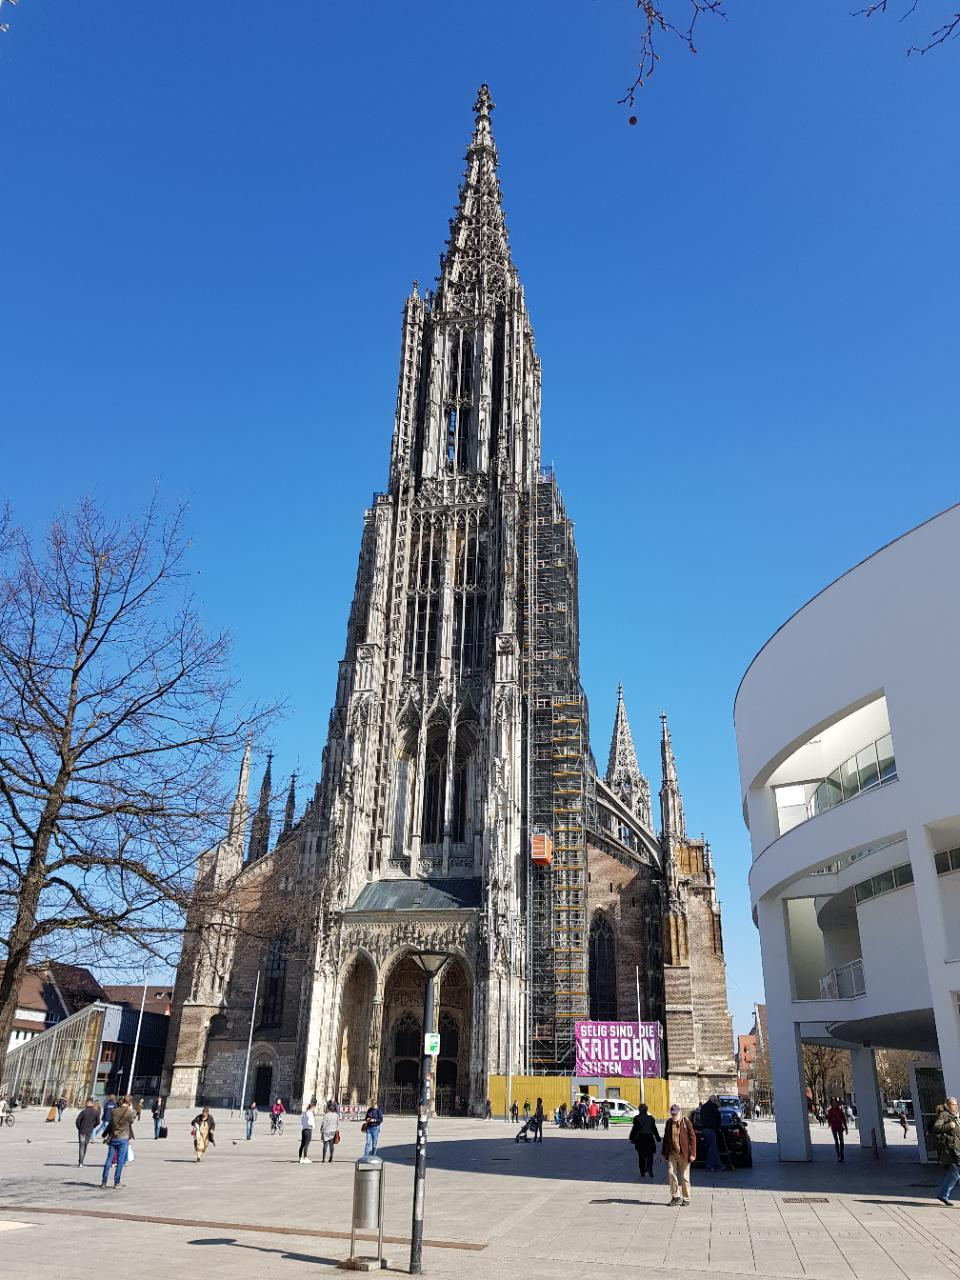
\includegraphics[width=.5\linewidth]{figures/ulm-minster.jpg}
  \caption{Ulmer Münster. Foto: wkrauth, CC0, via Wikimedia Commons.}
  \label{fig:jpg}
\end{figure}
\end{ltgexample}

\section{Sub Figures}

An example of two sub figures is shown in \zcref{fig:two_sub_figures}.

\begin{ltgexample}
\begin{figure}[!b]
  \centering
  \subfloat[Case I]{\includegraphics[width=.4\linewidth]{example-image-a}%
    \label{fig:first_case}}
  \hfil
  \subfloat[Case II]{\includegraphics[width=.4\linewidth]{example-image-b}%
    \label{fig:second_case}}
  \caption{Example figure with two sub figures.}
  \label{fig:two_sub_figures}
\end{figure}
\end{ltgexample}

\section{Figures with tikz}

The \href{https://ctan.org/pkg/pgf}{tikz} package creates graphics programmatically.
This package generates grids and other regular structures.

\begin{ltgexample}
\begin{figure}[ht]
  \centering
  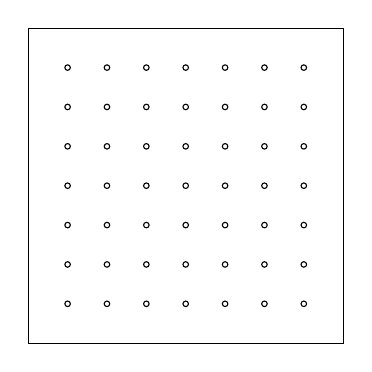
\begin{tikzpicture}
    \draw(0,0) rectangle (4,4);
    \foreach \x in {0.5,1,1.5,2,2.5,3,3.5}
    \foreach \y in {0.5,1,1.5,2,2.5,3,3.5}
    \draw(\x,\y) circle (1pt);
  \end{tikzpicture}
  \caption{A regular grid generated easily with two for loops.}\label{fig:tikz_example}
\end{figure}
\end{ltgexample}

\section{Plots with pgfplots}

The \href{https://ctan.org/pkg/pgfplots}{pgfplots} package plots functions directly in \LaTeX{}, similar to MATLAB or gnuplot.
Some visual examples are available in the package documentation\footnote{\url{http://texdoc.net/pkg/pgfplots}}.

\begin{ltgexample}
\begin{figure}[ht]
  \centering
  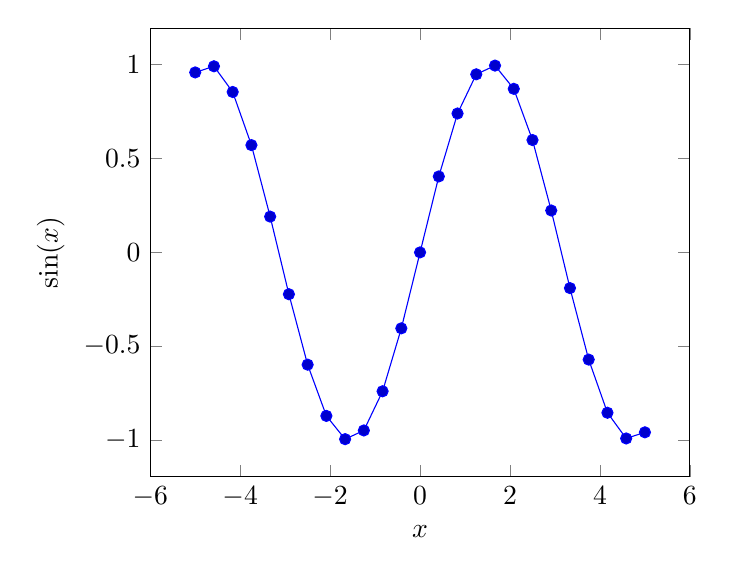
\begin{tikzpicture}
    \begin{axis}[xlabel=$x$, ylabel=$\sin(x)$]
      \addplot {sin(deg(x))};  % Plot the sine function
    \end{axis}
  \end{tikzpicture}
  \caption{Plot of $\sin(x)$ directly inside the figure environment with pgfplots.}
  \label{fig:pgfplots_example}
\end{figure}
\end{ltgexample}

Coordinates can also be given explicitly instead of as a function:
\begin{ltgexample}
\begin{figure}[ht]
  \centering
  \begin{tikzpicture}
    \begin{axis}[xlabel=$x$, ylabel=$y$]
      \addplot coordinates {(0,0) (1,1) (2,4) (3,9)};  % Plot explicit coordinates
    \end{axis}
  \end{tikzpicture}
  \caption{Explicit coordinates plotted with pgfplots.}
  \label{fig:pgfplots_coords}
\end{figure}
\end{ltgexample}

\section{UML diagrams}

UML diagrams can be written as text next to the \LaTeX{} source and are typeset in the fonts of the document.
\href{https://ctan.org/pkg/metauml}{MetaUML} draws class, component, and further diagrams.
It is MetaPost code, which \texttt{lualatex} runs itself via the \href{https://ctan.org/pkg/luamplib}{luamplib} package; no further tools are needed.
Thus, the MetaUML diagrams are shown only when compiling with \texttt{lualatex}.
The \href{https://ctan.org/pkg/pgf-umlsd}{pgf-umlsd} package draws sequence diagrams with TikZ and works with every engine.
A comparison of the packages for UML diagrams is given at \url{https://github.com/latextemplates/gadr-latex-packages/blob/main/uml-diagrams.md}.

\ifluatex
  \begin{ltgexample}
  \begin{figure}
    \centering
    \sffamily
    \begin{mplibcode}
      input metauml;
      beginfig(1);
      Class.Driver("Driver")()();
      Class.Car("Car")("+model: String")("+drive()");
      Class.Wheel("Wheel")()();
      Class.Person("Person")()();
      % distances between the boxes in PostScript points (1/72 inch)
      leftToRight(70)(Driver, Car, Wheel);
      topToBottom(50)(Car, Person);
      drawObjects(Driver, Car, Wheel, Person);
      link(association)(Driver.e -- Car.w);
      item(iAssoc)("drives >")(obj.s = .5[Driver.e, Car.w]);
      % the diamond is drawn at the end of the path
      link(composition)(Wheel.w -- Car.e);
      item(iAssoc)("have 4 >")(obj.s = .5[Car.e, Wheel.w]);
      link(association)(Car.s -- Person.n);
      item(iAssoc)("< owns")(obj.w = .5[Car.s, Person.n] + (5, 0));
      endfig;
    \end{mplibcode}
    \caption{Class diagram drawn with MetaUML}
    \label{fig:uml-class}
  \end{figure}
  \end{ltgexample}

  \begin{ltgexample}
  \begin{figure}
    \centering
    \sffamily
    \begin{mplibcode}
      input metauml;
      beginfig(1);
      Component.Client("Client")();
      Component.Server("Server")();
      % MetaUML has no automatic layout: each object is placed relative to another one;
      % here, the left edge of Server is 140 PostScript points (1/72 inch, about 5 cm) right of the right edge of Client
      Server.w = Client.e + (140, 0);
      drawObjects(Client, Server);
      % the interface: Server provides it (ball), Client requires it (socket)
      pair iface;
      iface = .5[Client.e, Server.w];
      link(providedInterface)(Server.w -- iface);
      link(requiredInterface)(Client.e -- iface);
      item(iAssoc)("API")(obj.s = iface + (0, 8));
      endfig;
    \end{mplibcode}
    \caption{Component diagram drawn with MetaUML}
    \label{fig:uml-component}
  \end{figure}
  \end{ltgexample}
\fi

\begin{ltgexample}
\begin{figure}
  \centering
  \sffamily
  \begin{sequencediagram}
    \newthread{client}{Client}
    % [3]: horizontal gap (in cm) to the box of the previous instance; the default (0.2) leaves no room for the message labels
    \newinst[3]{server}{Server}
    \begin{call}{client}{request()}{server}{response}
    \end{call}
  \end{sequencediagram}
  \caption{Sequence diagram drawn with pgf-umlsd}
  \label{fig:uml-sequence}
\end{figure}
\end{ltgexample}

\section{Tables}

\begin{ltgexample}
\begin{table}
  \caption{Simple Table}
  \label{tab:simple}
  \centering
  \begin{tabular}{ll}
    \toprule
    Heading1 & Heading2 \\
    \midrule
    One      & Two      \\
    Three    & Four     \\
    \bottomrule
  \end{tabular}
\end{table}
\end{ltgexample}

A table caption goes above the table (\verb|\caption| before the \verb|tabular|), a figure caption below the figure.

Rows and cells can be colored with \verb|\rowcolor| and \verb|\cellcolor| from the \href{https://ctan.org/pkg/colortbl}{colortbl} package, which \href{https://ctan.org/pkg/xcolor}{xcolor} loads with its option \verb|table|.

\begin{ltgexample}
\begin{table}
  \caption{Table with colored cells}
  \label{tab:colored}
  \centering
  \begin{tabular}{ll}
    \toprule
    \rowcolor{gray!20}
    Test & Result                   \\
    \midrule
    A    & \cellcolor{green!20}pass \\
    B    & \cellcolor{red!20}fail   \\
    \bottomrule
  \end{tabular}
\end{table}
\end{ltgexample}

A \verb|\footnote| inside a floating table is lost.
Use \verb|\tablefootnote| from the \href{https://ctan.org/pkg/tablefootnote}{tablefootnote} package instead: it is set as a normal footnote at the bottom of the page.
If the notes should appear directly below the table instead (common in journals), use the \href{https://ctan.org/pkg/threeparttable}{threeparttable} package.

\begin{ltgexample}
\begin{table}
  \caption{Table with a footnote}
  \label{tab:footnote}
  \centering
  \begin{tabular}{ll}
    \toprule
    Heading1 & Heading2\tablefootnote{A footnote inside a table.} \\
    \midrule
    One      & Two      \\
    \bottomrule
  \end{tabular}
\end{table}
\end{ltgexample}

\begin{ltgexample}
% Adapted from https://tex.stackexchange.com/a/468994/9075
\begin{table}
  \caption{Table with diagonal line}
  \label{tab:diag}
  \begin{center}
    \begin{tabular}{|l|c|c|}
      \hline
      \diagbox{Row}{Column} & A & B \\
      \hline
      1                     & x & y \\
      \hline
    \end{tabular}
  \end{center}
\end{table}
\end{ltgexample}


\section{Tables spanning multiple pages}

The \href{https://ctan.org/pkg/longtable}{longtable} package typesets tables that automatically break across page boundaries.
The header (\verb+\endhead+) and footer (\verb+\endfoot+) rows are repeated on every page; once enough rows are added, the table spans more than one page on its own.

\begin{ltgexample}
\begin{longtable}{|l|l|l|}
  \caption{A sample long table.}\label{tab:long} \\
  \hline
  \multicolumn{1}{|c|}{\textbf{First column}} & \multicolumn{1}{c|}{\textbf{Second column}} & \multicolumn{1}{c|}{\textbf{Third column}} \\ \hline
  \endfirsthead

  \multicolumn{3}{c}{{\bfseries \tablename\ \thetable{} -- continued from previous page}} \\
  \hline
  \multicolumn{1}{|c|}{\textbf{First column}} & \multicolumn{1}{c|}{\textbf{Second column}} & \multicolumn{1}{c|}{\textbf{Third column}} \\ \hline
  \endhead

  \hline \multicolumn{3}{|r|}{{Continued on next page}} \\ \hline
  \endfoot

  \hline\hline
  \endlastfoot

  A & BC & D \\
  A & BC & D \\
  A & BC & D \\
  A & BC & D \\
  A & BC & D \\
  A & BC & D \\
  A & BC & D \\
  A & BC & D \\
  A & BC & D \\
  A & BC & D \\
  A & BC & D \\
  A & BC & D \\
\end{longtable}
\end{ltgexample}

% The main file loads either the minted or the listings package
\ifdefined\inputminted
  \section{Source Code}

The \href{https://github.com/gpoore/minted}{minted} package highlights listings properly.
It uses the \href{http://pygments.org/}{pygments} library, which in turn requires Python.

\begin{ltgexample}
\Zcref{lst:XML} shows source code written in XML.
\Zcref{line:comment} contains a comment.

\begin{listing}[htbp]
  \begin{minted}[linenos=true,escapeinside=||]{xml}
<listing name="example">
  <!-- comment --> |\label{line:comment}|
  <content>not interesting</content>
</listing>
\end{minted}
  \caption{Example XML listing using minted}
  \label{lst:XML}
\end{listing}
\end{ltgexample}

One can also typeset JSON as shown in \zcref{lst:flJSON}.

\begin{ltgexample}
\begin{listing}[htbp]
  \begin{minted}[linenos=true,escapeinside=||]{json}
{
  key: "value"
}
\end{minted}
  \caption{Example JSON listing using minted}
  \label{lst:flJSON}
\end{listing}
\end{ltgexample}

Java is also possible as shown in \zcref{lst:flJava}.

\begin{ltgexample}
\begin{listing}[htbp]
  \begin{minted}[linenos=true,escapeinside=||]{java}
public class Hello {
    public static void main (String[] args) {
        System.out.println("Hello World!");
    }
}
\end{minted}
  \caption{Java code rendered using minted}
  \label{lst:flJava}
\end{listing}
\end{ltgexample}

Listings longer than the remaining space continue on the next page if they are \emph{not} floating.
A floating listing is always placed on a single page.
Thus, use \verb+\captionof{listing}+ instead of the \verb+listing+ environment.
\Zcref{lst:long} spans multiple pages.

\begin{minted}[linenos=true]{java}
public class Squares {

    /** Returns the square of 1. */
    public int square1() {
        return 1 * 1;
    }

    /** Returns the square of 2. */
    public int square2() {
        return 2 * 2;
    }

    /** Returns the square of 3. */
    public int square3() {
        return 3 * 3;
    }

    /** Returns the square of 4. */
    public int square4() {
        return 4 * 4;
    }

    /** Returns the square of 5. */
    public int square5() {
        return 5 * 5;
    }

    /** Returns the square of 6. */
    public int square6() {
        return 6 * 6;
    }

    /** Returns the square of 7. */
    public int square7() {
        return 7 * 7;
    }

    /** Returns the square of 8. */
    public int square8() {
        return 8 * 8;
    }

    /** Returns the square of 9. */
    public int square9() {
        return 9 * 9;
    }

    /** Returns the square of 10. */
    public int square10() {
        return 10 * 10;
    }

    /** Returns the square of 11. */
    public int square11() {
        return 11 * 11;
    }

    /** Returns the square of 12. */
    public int square12() {
        return 12 * 12;
    }

    public static void main(String[] args) {
        System.out.println(new Squares().square12());
    }
}
\end{minted}
\captionof{listing}{Long Java listing spanning multiple pages}
\label{lst:long}

\else
  \section{Quellcode}

\begin{ltgexample}
\Zcref{lst:XML} zeigt XML-Quelltext.
\Zcref{line:comment} enthält einen Kommentar.

\begin{lstlisting}[
  language=XML,
  caption={Beispiel-XML-Listing},
  label={lst:XML}]
<listing name="example">
  <!-- comment --> (* \label{line:comment} *)
  <content>not interesting</content>
</listing>
\end{lstlisting}
\end{ltgexample}

Der zusätzliche Parameter \verb+float+ führt dazu, dass das Listing auch floated.
\Zcref{lst:flXML} zeigt das gleitende Listing.

\begin{ltgexample}
\begin{lstlisting}[
  % Es ist möglcih, die Abstände bei Bedarf einzustellen
  % aboveskip=2.5\baselineskip,
  % belowskip=-.8\baselineskip,
  float,
  language=XML,
  caption={Beispiel-XML-Listing -- gleitend},
  label={lst:flXML}]
<listing name="example">
  Floating
</listing>
\end{lstlisting}
\end{ltgexample}

Es ist möglich auch JSON zu setzen, wie in \zcref{lst:json} gezeigt.

\begin{ltgexample}
\begin{lstlisting}[
  float,
  language=json,
  caption={Beispiel-JSON-listing},
  label={lst:json}]
{
  key: "value"
}
\end{lstlisting}
\end{ltgexample}

Java ist auch möglich -- \zcref{lst:java}.

\begin{ltgexample}
\begin{lstlisting}[
  caption={Example Java listing},
  label=lst:java,
  language=Java,
  float]
public class Hello {
    public static void main (String[] args) {
        System.out.println("Hello World!");
    }
}
\end{lstlisting}
\end{ltgexample}

Listings longer than the remaining space continue on the next page if they are \emph{not} floating.
A floating listing is always placed on a single page.
\Zcref{lst:long} spans multiple pages.

\begin{lstlisting}[
  language=Java,
  caption={Long Java listing spanning multiple pages},
  label={lst:long}]
public class Squares {

    /** Returns the square of 1. */
    public int square1() {
        return 1 * 1;
    }

    /** Returns the square of 2. */
    public int square2() {
        return 2 * 2;
    }

    /** Returns the square of 3. */
    public int square3() {
        return 3 * 3;
    }

    /** Returns the square of 4. */
    public int square4() {
        return 4 * 4;
    }

    /** Returns the square of 5. */
    public int square5() {
        return 5 * 5;
    }

    /** Returns the square of 6. */
    public int square6() {
        return 6 * 6;
    }

    /** Returns the square of 7. */
    public int square7() {
        return 7 * 7;
    }

    /** Returns the square of 8. */
    public int square8() {
        return 8 * 8;
    }

    /** Returns the square of 9. */
    public int square9() {
        return 9 * 9;
    }

    /** Returns the square of 10. */
    public int square10() {
        return 10 * 10;
    }

    /** Returns the square of 11. */
    public int square11() {
        return 11 * 11;
    }

    /** Returns the square of 12. */
    public int square12() {
        return 12 * 12;
    }

    public static void main(String[] args) {
        System.out.println(new Squares().square12());
    }
}
\end{lstlisting}

\fi

\section{Itemization}

One can list items as follows:

\begin{ltgexample}
\begin{itemize}
  \item Item One
  \item Item Two
\end{itemize}
\end{ltgexample}

With the package paralist, one can create itemizations with lesser spacing:

\begin{ltgexample}
\begin{compactitem}
  \item Item One
  \item Item Two
\end{compactitem}
\end{ltgexample}

One can enumerate items as follows:

\begin{ltgexample}
\begin{enumerate}
  \item Item One
  \item Item Two
\end{enumerate}
\end{ltgexample}

With the package paralist, one can create enumerations with lesser spacing:

\begin{ltgexample}
\begin{compactenum}
  \item Item One
  \item Item Two
\end{compactenum}
\end{ltgexample}

With paralist, one can even have all items typeset after each other and have them clean in the TeX document:

\begin{ltgexample}
\begin{inparaenum}
  \item The first item,
  \item the second item, and
  \item the third item appear in one line.
\end{inparaenum}
\end{ltgexample}

\section{Writing in Markdown}\label{sec:markdown}

\ifluatex
  If you are new to \LaTeX{}, you can start by writing your text in Markdown using the \href{https://ctan.org/pkg/markdown}{markdown} package.
  \LaTeX{} then takes care of the typesetting.
  Markdown and \LaTeX{} can be mixed:
  \Zcref{tbl:markdown} is written in Markdown and referenced from \LaTeX{}.
  A whole chapter can be written in a separate Markdown file included by \verb|\markdownInput|, as \zcref{sec:markdown-file} shows.
  The \href{https://github.com/latextemplates/markdown-latex-quickstart}{markdown-latex-quickstart} shows a complete document written in Markdown.

  \begin{ltgexample}
  \begin{markdown}
Text can be *emphasized* or **bold**, and `code` is set in a monospaced font.
A citation looks like this [@mwe], and here is a footnote.^[This is an inline footnote.]

- first point
- second point
  - sub-point

1) firstly
2) secondly

| Right | Left | Centered |
|------:|:-----|:--------:|
|    12 | 12   |    12    |
|   123 | 123  |   123    |

: A table written in Markdown {#tbl:markdown}

<#tbl:markdown> shows a table with caption.
Its identifier `{#tbl:markdown}` is referenced by `<#tbl:markdown>`.
\end{markdown}
  \end{ltgexample}
\else
  This example requires \hologo{LuaLaTeX}.
  Compile the document with \hologo{LuaLaTeX} to see it.
\fi

\section{Abkürzungen}

Mit \verb+\gls{...}+ können Abkürzungen eingebaut werden, beim ersten Aufrufen wird die lange Form eingesetzt.
Beim wiederholten Verwenden von \verb+\gls{...}+ wird automatisch die Kurzform angezeigt.
Außerdem wird die Abkürzung automatisch in die Abkürzungsliste eingefügt.
Mit \verb+\glspl{...}+ wird die Pluralform verwendet.
Möchte man, dass bei der ersten Verwendung direkt die Kurzform erscheint, so kann man mit \verb+\glsunset{...}+ eine Abkürzung als bereits verwendet markieren.
Das Gegenteil erreicht man mit \verb+\glsreset{...}+.

Definiert werden Abkürzungen in der Datei \textit{abbreviationstex} mithilfe von \verb+\newacronym{...}{...}{...}+.

Mehr Infos unter: \url{https://ctan.org/pkg/bib2gls}.

\begin{ltgexample}
Beim ersten Durchlauf betrug die \gls{fr} 5.
Beim zweiten Durchlauf war die \gls{fr} 3.
Die Pluralform sieht man hier: \glspl{fr}.
Um zu demonstrieren, wie das Abkürzungsverzeichnis bei längeren Beschreibungstexten aussieht, muss hier noch \glspl{rdbms} erwähnt werden.

\gls{dante} is a local \TeX\ user group.
The German-speaking local \TeX\ user group is \gls{dante}.
A \gls{gp} is a medical doctor.
I went to my surgery to see the \gls{gp}.
\end{ltgexample}

\section{Other Features}

\begin{ltgexample}
The words \enquote{workflow} and \enquote{dwarflike} can be copied from the PDF and pasted to a text file.
\end{ltgexample}

\begin{ltgexample}
The symbol for powerset is now correct: $\powerset$ and not a Weierstrass p ($\wp$).

$\powerset({1,2,3})$
\end{ltgexample}

\begin{ltgexample}
Brackets work as designed:
<test>
One can also input backticks in verbatim text: \verb|`test`|.
\end{ltgexample}

Acronyms can be typeset in running text with \verb+\initialism+, which sets them as small caps that blend into the surrounding lowercase text. It is the lightweight alternative to the full acronym and glossary management (\verb+\gls+, with an automatic list of abbreviations) provided by the thesis variants: \verb+\initialism+ only typesets the acronym and does not add it to any list. The macro and the ready-made acronyms (\verb+\OMG+, \verb+\BPEL+, \verb+\BPMN+, \verb+\UML+) are defined in \texttt{commands.tex}, where you can add your own.

\begin{ltgexample}
The \UML is maintained by the \OMG; related standards include \BPEL and \BPMN.
Any acronym can be set inline with \initialism{REST} or \initialism{HTTP}.
\end{ltgexample}


\section{Zref-vario examples}
\label{sec:ex:vref}

Demonstration of zref-vario: zvref[S] at the beginning of a sentence, zvref in all other cases.

\begin{ltgexample}
\zvref[S]{fig:ex:cref} shows a simple fact, although \zvref{fig:ex:cref} could also show something else.

\zvref[S]{tab:ex:cref} shows a simple fact, although \zvref{tab:ex:cref} could also show something else.

\zvref[S]{sec:ex:cref} shows a simple fact, although \zvref{sec:ex:cref} could also show something else.
\end{ltgexample}

\section{Citations}

When referencing something from the bibliography file, it will automatically appear in the references section.
If a reference is not cited, it is not appearing there.

\begin{ltgexample}
Standard case: Citing indirectly citing something~\cite{mwe}.
In case one wants to name the author: \textcite{mwe} shows a minimal \LaTeX{} example.
\end{ltgexample}

Note that \texttt{\textbackslash textcite\{mwe\}} prints both the author and the reference to the bibliography entry.

A thesis is cited like any other work: a master's thesis~\cite{Shannon1940} or a doctoral thesis~\cite{Nash1950}.
The entry types \texttt{@MastersThesis} and \texttt{@PhdThesis} are labeled in the document language (\enquote{MA thesis} or \enquote{Masterarbeit}, \enquote{PhD thesis} or \enquote{Diss.}).
For a Bachelor's thesis, use \texttt{@Thesis} with \texttt{type = \{bathesis\}}; for a Diplomarbeit, \texttt{type = \{Diplomarbeit\}} is printed as is.

Remember that you have to call \texttt{biber main-german} to generate the bibliography data for \texttt{lualatex}.
You will need to run \texttt{lualatex} twice so that the page numbers are up to date.


In the bibliography, use \texttt{\textbackslash textsuperscript} for \enquote{st}, \enquote{nd}, \ldots:
E.g., \enquote{The 2\textsuperscript{nd} conference on examples}.
When you use \href{https://www.jabref.org}{JabRef}, you can use the cleanup command to achieve that.
See \url{https://help.jabref.org/en/CleanupEntries} for an overview of the cleanup functionality.

\section{Miscellaneous Examples}
\label{ssec:example}

Reference test: \Zcref{ssec:example}, \zcref{fig:Abbildung} and \zcref{alg:example}.

\begin{ltgexample}
Checkmark: \dingcheck.
Crossmark: \dingcross.
\end{ltgexample}

\begin{figure}
  \missingfigure{}
  \caption{Figure}
  \label{fig:Abbildung}
\end{figure}

\begin{landscape}
  \begin{figure}
    \missingfigure{}
    \caption{Rotated figure}
    \label{fig:AbbildungGedreht}
  \end{figure}
\end{landscape}

\subsection{Algorithms}

\begin{algorithm}
  \caption{$algo$}
  \label{alg:example}
  \begin{algorithmic}[1]
    \State $a \gets 0$
    \State State 2\label{alg1:state2}
  \end{algorithmic}
\end{algorithm}

\begin{algorithm}
  \caption{Algorithm 2}
  \label{alg:example2}
  \begin{algorithmic}[1]
    \State $a \gets 0$
    \State State 2\label{alg2:state2}
  \end{algorithmic}
\end{algorithm}

\Zcref{alg:example} has already shown an algorithm.
Test of line referencing: line~\ref{alg1:state2} (\zcref{alg:example}) and line~\ref{alg2:state2} (\zcref{alg:example2}).

\subsection{Definitions}
\begin{definition}[Title]
  \label{def:def1}
  Definition Text
\end{definition}

\Zcref{def:def1} shows \ldots

\subsection{Enumerations}

\begin{enumerate}[label=\alph*)]
  \item a
  \item b
  \item c
  \item d
\end{enumerate}

Equivalent to paralist's inparaenum:
\begin{enumerate*}[label=\alph*)]
  \item a
  \item b
  \item c
  \item d
\end{enumerate*}

\begin{description}
  \item[first] First
  \item[second] Second
  \item[third] Third
\end{description}

\begin{description}
  \item[\texttt{first}] First
  \item[\texttt{second}] Second
  \item[\texttt{third}] Third
\end{description}

%works only if package enumitem is loaded
\begin{description}[font=\ttfamily]
  \item[first] First
  \item[second] Second
  \item[third] Third
\end{description}

\begin{description}[style=unboxed]
  \item[first label with a long description text breaking over one line. Enabled by the enumitem package] First
  \item[second] Second
  \item[third] Third
\end{description}

\begin{Description}
  \item[first label with a long description text breaking over one line. Defined in the template] First
  \item[second] Second
  \item[third] Third
\end{Description}

\begin{itemize}
  \item First
  \item Second
  \item Third
\end{itemize}

The optional parameter changes the marker that is prepended.
See \url{http://www.weinelt.de/latex/item.html}.
\begin{itemize}
  \item[A] First
  \item[B] Second
  \item[C] Third
\end{itemize}

Incorrect use of the optional parameter as follows:
\begin{itemize}
  \item[first] First
  \item[second] Second
  \item[third] Third
\end{itemize}
Note that, when \texttt{enumitem} is loaded, this behaves differently than with \texttt{paralist}.

\subsection{The fquote environment}

\begin{fquote}[T.\ Scientist]
  The program will be finished by next Friday.
\end{fquote}

\begin{gfquote}{T.\ Scientist}
  The program will be finished by next Friday.
\end{gfquote}

% Compiles on its own: latexmk "90 - zusammenfassung" (in this directory, see README.md).
% The subfiles package loads the preamble of the main file named here.
\documentclass[../main-german]{subfiles}
%\documentclass[../main-basic-listings-german]{subfiles}
%\documentclass[../main-german-thu]{subfiles}
%\documentclass[../main-german-university-of-hamburg]{subfiles}
\begin{document}
%%% ===============================================================================
\chapter{Zusammenfassung und Ausblick}\label{sec:conclusion}
%%% ===============================================================================
\progress{0}

Your conclusions are more than a factual summary of your work: they position, interpret, and defend your findings against the state of the art that you discussed in \zcref{sec:introduction:state-of-art}.
You specifically outline which concrete findings or methodological contributions advance our knowledge towards the general objective you introduced in \zcref{sec:introduction:topic}.
Objectively discuss which parts you solved and in which parts you failed.

You should explicitly discuss limitations and shortcomings of your work and detail what kind of future studies are needed to overcome these limitations.
Be specific in the sense that your arguments for future work should be based on concrete findings and insights you obtained in your report.
\end{document}


%%% ===============================================================================
%%% Bibliography
%%% ===============================================================================


\printbibliography

% Enforce empty line after bibliography
\ \\
%
\noindent
Alle Links wurden zuletzt am 29.03.2021 geprüft.

%%% ===============================================================================

%\IfDefined{printindex}{\printindex}
%\IfDefined{printnomenclature}{\printnomenclature}

\clearpage
\appendix
% 'Anhang' ins Inhaltsverzeichnis
%\phantomsection
%\addcontentsline{toc}{chapter}{Anhang}
\addcontentsline{toc}{part}{Anhang}

%%% ===============================================================================
\chapter{My first appendix}\label{sec:appendix1}
%%% ===============================================================================

\lipsum[1]

%%% ===============================================================================
\chapter{Nutzung von KI-Tools}\label{sec:ai-tools}
%%% ===============================================================================

% Hier wird dokumentiert, inwiefern KI-Tools zur Erstellung wesentlicher Teile dieser Arbeit verwendet wurden.
% Die Struktur ist mit der Prüferin oder dem Prüfer abzustimmen.
% Nur übernommene KI-Outputs (z.B. Text, Abbildungen) müssen aufgeführt werden; die Nutzung von KI zur Recherche oder Rechtschreibprüfung nicht.
% Wurden keine KI-Outputs als wesentliche Teile übernommen, ist dies statt der Tabelle zu erklären.

\begin{tabular}{lll}
  \toprule
  KI-Tool          & Genutzt für                    & Genutzt in                \\
  \midrule
  ChatGPT5         & Erstellung von Abbildungen     & \zcref{fig:label,fig:jpg} \\
  Google AI search & Pseudocode für Algorithmus XYZ & \zcref{alg:example}       \\
  DeepL Write      & Umformulierung der Einleitung  & \zcref{sec:introduction}  \\
  \bottomrule
\end{tabular}

\pagestyle{empty}
\renewcommand*{\chapterpagestyle}{empty}
\clearpage
\backmatter
\thispagestyle{empty}

\vspace*{\fill}
\pagestyle{empty}

% textidote: ignore begin
{\normalsize
  \begin{center}\textbf{Eidesstattliche Erklärung}\end{center}
  \blindtext[1]
  \vspace*{1cm}\\
  Ulm, den XX.XX.20XX
  \hspace*{\fill}\begin{tabular}{@{}l@{}}\hline
    \makebox[5cm]{Vorname Nachname}
  \end{tabular}
  \vspace*{3cm}

  %TODO Dies ist optional, ggf. löschen!
  \begin{center}\textbf{Veröffentlichung}\end{center}
  \blindtext[1]
  \vspace*{1cm}\\
  Ulm, den XX.XX.20XX
  \hspace*{\fill}\begin{tabular}{@{}l@{}}\hline
    \makebox[5cm]{Vorname Nachname}
  \end{tabular}
}
% textidote: ignore end
\vspace*{\fill}
\end{document}
